% !TEX root = z_output/_Riehl.tex

\documentclass[11pt]{article}
\usepackage{fullpage}
\usepackage{amsmath,amsthm,amssymb}
\usepackage{mathrsfs,nicefrac}
\usepackage{amssymb}
\usepackage{epsfig}
\usepackage[all]{xy}
\usepackage{sseq}
\usepackage{tocloft}
\usepackage{cancel}
\usepackage[strict]{changepage}
\usepackage{color}
\usepackage{tikz}
\usepackage{extpfeil}
\usepackage{version}
%\usepackage{ifthen}
%Used for disabling hyperref
\ifx\dontloadhyperref\undefined
%\usepackage[pdftex,pdfborder={0 0 0 [1 1]}]{hyperref}
\usepackage[pdftex,pdfborder={0 0 .5 [1 1]}]{hyperref}
\else
\providecommand{\texorpdfstring}[2]{#1}
\fi

%>>>>>>>>>>>>>>>>>>>>>>>>>>>>>>
%<<<       Better ToC       <<<
%>>>>>>>>>>>>>>>>>>>>>>>>>>>>>>
\setlength{\cftbeforesecskip}{0.5ex}

%>>>>>>>>>>>>>>>>>>>>>>>>>>>>>>
%<<<      Hyperref mod      <<<
%>>>>>>>>>>>>>>>>>>>>>>>>>>>>>>

%needs more testing
\newcounter{dummyforrefstepcounter}
\newcommand{\labelRIGHTHERE}[1]
{\refstepcounter{dummyforrefstepcounter}\label{#1}}


%>>>>>>>>>>>>>>>>>>>>>>>>>>>>>>
%<<<  Theorem Environments  <<<
%>>>>>>>>>>>>>>>>>>>>>>>>>>>>>>
\ifx\dontloaddefinitionsoftheoremenvironments\undefined
\theoremstyle{plain}
\newtheorem{thm}{Theorem}[section]
\newtheorem*{thm*}{Theorem}
\newtheorem{lem}[thm]{Lemma}
\newtheorem*{lem*}{Lemma}
\newtheorem{prop}[thm]{Proposition}
\newtheorem*{prop*}{Proposition}
\newtheorem{cor}[thm]{Corollary}
\newtheorem*{cor*}{Corollary}
\newtheorem{defprop}[thm]{Definition-Proposition}
\newtheorem*{punchline}{Punchline}

\theoremstyle{definition}
\newtheorem{defn}{Definition}[section]
\newtheorem*{defn*}{Definition}
\newtheorem{exmp}{Example}[section]
\newtheorem*{exmp*}{Example}
\newtheorem{asspt}{Assumption}[section]
\newtheorem{notation}{Notation}[section]
\newtheorem{exercise}{Exercise}[section]
\newtheorem*{fact*}{Fact}
\newtheorem*{rmk*}{Remark}
\newtheorem{fact}{Fact}
\newtheorem*{aside}{Aside}
\newtheorem*{question}{Question}
\newtheorem*{answer}{Answer}

\else\relax\fi

%>>>>>>>>>>>>>>>>>>>>>>>>>>>>>>
%<<<      Fields, etc.      <<<
%>>>>>>>>>>>>>>>>>>>>>>>>>>>>>>
\DeclareSymbolFont{AMSb}{U}{msb}{m}{n}
\DeclareMathSymbol{\N}{\mathbin}{AMSb}{"4E}
\DeclareMathSymbol{\Octonions}{\mathbin}{AMSb}{"4F}
\DeclareMathSymbol{\Z}{\mathbin}{AMSb}{"5A}
\DeclareMathSymbol{\R}{\mathbin}{AMSb}{"52}
\DeclareMathSymbol{\Q}{\mathbin}{AMSb}{"51}
\DeclareMathSymbol{\PP}{\mathbin}{AMSb}{"50}
\DeclareMathSymbol{\I}{\mathbin}{AMSb}{"49}
\DeclareMathSymbol{\C}{\mathbin}{AMSb}{"43}
\DeclareMathSymbol{\A}{\mathbin}{AMSb}{"41}
\DeclareMathSymbol{\F}{\mathbin}{AMSb}{"46}
\DeclareMathSymbol{\Quaternions}{\mathbin}{AMSb}{"48}


%>>>>>>>>>>>>>>>>>>>>>>>>>>>>>>
%<<<       Operators        <<<
%>>>>>>>>>>>>>>>>>>>>>>>>>>>>>>
\DeclareMathOperator{\ad}{\textbf{ad}}
\DeclareMathOperator{\coker}{coker}
\renewcommand{\ker}{\textup{ker}\,}
\DeclareMathOperator{\End}{End}
\DeclareMathOperator{\Aut}{Aut}
\DeclareMathOperator{\Hom}{Hom}
\DeclareMathOperator{\Maps}{Maps}
\DeclareMathOperator{\Mor}{Mor}
\DeclareMathOperator{\Gal}{Gal}
\DeclareMathOperator{\Ext}{Ext}
\DeclareMathOperator{\Tor}{Tor}
\DeclareMathOperator{\Map}{Map}
\DeclareMathOperator{\Der}{Der}
\DeclareMathOperator{\Rad}{Rad}
\DeclareMathOperator{\rank}{rank}
\DeclareMathOperator{\ArfInvariant}{Arf}
\DeclareMathOperator{\KervaireInvariant}{Ker}
\DeclareMathOperator{\im}{im}
\DeclareMathOperator{\coim}{coim}
\DeclareMathOperator{\trace}{tr}
\DeclareMathOperator{\supp}{supp}
\DeclareMathOperator{\ann}{ann}
\DeclareMathOperator{\spec}{Spec}
\DeclareMathOperator{\proj}{Proj}
\DeclareMathOperator{\fiber}{F}
\DeclareMathOperator{\cofiber}{C}
\DeclareMathOperator{\cone}{cone}
\DeclareMathOperator{\Skel}{Sk}
\DeclareMathOperator{\conn}{conn}
\DeclareMathOperator{\colim}{colim}
\DeclareMathOperator{\limit}{lim}

%>>>>>>>>>>>>>>>>>>>>>>>>>>>>>>
%<<<   Cohomology Theories  <<<
%>>>>>>>>>>>>>>>>>>>>>>>>>>>>>>
\DeclareMathOperator{\KR}{{K\R}}
\DeclareMathOperator{\KO}{{KO}}
\DeclareMathOperator{\K}{{K}}
\DeclareMathOperator{\OmegaO}{{\Omega_{\Octonions}}}

%>>>>>>>>>>>>>>>>>>>>>>>>>>>>>>
%<<<   Algebraic Geometry   <<<
%>>>>>>>>>>>>>>>>>>>>>>>>>>>>>>
\DeclareMathOperator{\Spec}{Spec}
\DeclareMathOperator{\Proj}{Proj}
\DeclareMathOperator{\Sing}{Sing}
\DeclareMathOperator{\shfHom}{\mathscr{H}\textit{\!\!om}}
\newcommand{\WeilDivisors}{\textup{Div}}
\newcommand{\CartierDivisors}{\textup{CaDiv}}
\newcommand{\PrincipalWeilDivisors}{\textup{PrDiv}}
\newcommand{\LocallyPrincipalWeilDivisors}{\textup{LPDiv}}
\newcommand{\PrincipalCartierDivisors}{\textup{PrCaDiv}}
\newcommand{\DivisorClass}{\textup{Cl}}
\newcommand{\CartierClass}{\textup{CaCl}}
\newcommand{\Picard}{\textup{Pic}}
\DeclareMathOperator{\Frob}{Frob}


%>>>>>>>>>>>>>>>>>>>>>>>>>>>>>>
%<<<  Mathematical Objects  <<<
%>>>>>>>>>>>>>>>>>>>>>>>>>>>>>>
\newcommand{\sll}{\mathfrak{sl}}
\newcommand{\gl}{\mathfrak{gl}}
\newcommand{\GL}{\mbox{GL}}
\newcommand{\PGL}{\mbox{PGL}}
\newcommand{\SL}{\mbox{SL}}
\newcommand{\Mat}{\mbox{Mat}}
\newcommand{\Gr}{\textup{Gr}}
\newcommand{\Squ}{\textup{Sq}}
\newcommand{\catSet}{\textit{Sets}}
\newcommand{\RP}{{\R\PP}}
\newcommand{\CP}{{\C\PP}}
\newcommand{\Steen}{\mathscr{A}}
\newcommand{\Orth}{\textup{\textbf{O}}}

%>>>>>>>>>>>>>>>>>>>>>>>>>>>>>>
%<<<  Mathematical Symbols  <<<
%>>>>>>>>>>>>>>>>>>>>>>>>>>>>>>
\newcommand{\DASH}{\textup{---}}
\newcommand{\op}{\textup{op}}
\newcommand{\ob}{\textup{ob}\,}
\newcommand{\ho}{\textup{ho}}
\newcommand{\st}{\textup{st}}
\newcommand{\id}{\textup{id}}
\newcommand{\Bullet}{\ensuremath{\bullet} }

%>>>>>>>>>>>>>>>>>>>>>>>>>>>>>>
%<<<      Some Arrows       <<<
%>>>>>>>>>>>>>>>>>>>>>>>>>>>>>>
\let\shortmapsto\mapsto
\let\mapsto\longmapsto
\newcommand{\mapsfrom}{\,\reflectbox{$\mapsto$}\ }
\newcommand{\bigrightsquig}{\scalebox{2}{\ensuremath{\rightsquigarrow}}}
\newcommand{\bigleftsquig}{\reflectbox{\scalebox{2}{\ensuremath{\rightsquigarrow}}}}

%\newcommand{\cofibration}{\xhookrightarrow{\phantom{\ \,{\sim\!}\ \ }}}
%\newcommand{\fibration}{\xtwoheadrightarrow{\phantom{\sim\!}}}
%\newcommand{\acycliccofibration}{\xhookrightarrow{\ \,{\sim\!}\ \ }}
%\newcommand{\acyclicfibration}{\xtwoheadrightarrow{\sim\!}}
%\newcommand{\leftcofibration}{\xhookleftarrow{\phantom{\ \,{\sim\!}\ \ }}}
%\newcommand{\leftfibration}{\xtwoheadleftarrow{\phantom{\sim\!}}}
%\newcommand{\leftacycliccofibration}{\xhookleftarrow{\ \ {\sim\!}\,\ }}
%\newcommand{\leftacyclicfibration}{\xtwoheadleftarrow{\sim\!}}
%\newcommand{\weakequiv}{\xrightarrow{\ \,\sim\,\ }}
%\newcommand{\leftweakequiv}{\xleftarrow{\ \,\sim\,\ }}

\newcommand{\cofibration}
{\xhookrightarrow{\phantom{\ \,{\raisebox{-.3ex}[0ex][0ex]{\scriptsize$\sim$}\!}\ \ }}}
\newcommand{\fibration}
{\xtwoheadrightarrow{\phantom{\raisebox{-.3ex}[0ex][0ex]{\scriptsize$\sim$}\!}}}
\newcommand{\acycliccofibration}
{\xhookrightarrow{\ \,{\raisebox{-.55ex}[0ex][0ex]{\scriptsize$\sim$}\!}\ \ }}
\newcommand{\acyclicfibration}
{\xtwoheadrightarrow{\raisebox{-.6ex}[0ex][0ex]{\scriptsize$\sim$}\!}}
\newcommand{\leftcofibration}
{\xhookleftarrow{\phantom{\ \,{\raisebox{-.3ex}[0ex][0ex]{\scriptsize$\sim$}\!}\ \ }}}
\newcommand{\leftfibration}
{\xtwoheadleftarrow{\phantom{\raisebox{-.3ex}[0ex][0ex]{\scriptsize$\sim$}\!}}}
\newcommand{\leftacycliccofibration}
{\xhookleftarrow{\ \ {\raisebox{-.55ex}[0ex][0ex]{\scriptsize$\sim$}\!}\,\ }}
\newcommand{\leftacyclicfibration}
{\xtwoheadleftarrow{\raisebox{-.6ex}[0ex][0ex]{\scriptsize$\sim$}\!}}
\newcommand{\weakequiv}
{\xrightarrow{\ \,\raisebox{-.3ex}[0ex][0ex]{\scriptsize$\sim$}\,\ }}
\newcommand{\leftweakequiv}
{\xleftarrow{\ \,\raisebox{-.3ex}[0ex][0ex]{\scriptsize$\sim$}\,\ }}


%>>>>>>>>>>>>>>>>>>>>>>>>>>>>>>
%<<<     Greek Letters      <<<
%>>>>>>>>>>>>>>>>>>>>>>>>>>>>>>
%\newcommand{\oldphi}{\phi}
%\renewcommand{\phi}{\varphi}
\let\oldphi\phi
\let\phi\varphi
\renewcommand{\to}{\longrightarrow}
\newcommand{\eps}{\varepsilon}

%>>>>>>>>>>>>>>>>>>>>>>>>>>>>>>
%<<<  1st-4th & parentheses <<<
%>>>>>>>>>>>>>>>>>>>>>>>>>>>>>>
\newcommand{\first}{^\text{st}}
\newcommand{\second}{^\text{nd}}
\newcommand{\third}{^\text{rd}}
\newcommand{\fourth}{^\text{th}}
\newcommand{\ZEROTH}{$0^\text{th}$ }
\newcommand{\FIRST}{$1^\text{st}$ }
\newcommand{\SECOND}{$2^\text{nd}$ }
\newcommand{\THIRD}{$3^\text{rd}$ }
\newcommand{\FOURTH}{$4^\text{th}$ }
\newcommand{\iTH}{$i^\text{th}$ }
\newcommand{\jTH}{$j^\text{th}$ }
\newcommand{\nTH}{$n^\text{th}$ }

%>>>>>>>>>>>>>>>>>>>>>>>>>>>>>>
%<<<    upright commands    <<<
%>>>>>>>>>>>>>>>>>>>>>>>>>>>>>>
\newcommand{\upcol}{\textup{:}}
\newcommand{\upsemi}{\textup{;}}
\providecommand{\lparen}{\textup{(}}
\providecommand{\rparen}{\textup{)}}
\renewcommand{\lparen}{\textup{(}}
\renewcommand{\rparen}{\textup{)}}
\newcommand{\Iff}{\emph{iff} }

%>>>>>>>>>>>>>>>>>>>>>>>>>>>>>>
%<<<     Environments       <<<
%>>>>>>>>>>>>>>>>>>>>>>>>>>>>>>
\newcommand{\squishlist}
{ %\setlength{\topsep}{100pt} doesn't seem to do anything.
  \setlength{\itemsep}{.5pt}
  \setlength{\parskip}{0pt}
  \setlength{\parsep}{0pt}}
\newenvironment{itemise}{
\begin{list}{\textup{$\rightsquigarrow$}}
   {  \setlength{\topsep}{1mm}
      \setlength{\itemsep}{1pt}
      \setlength{\parskip}{0pt}
      \setlength{\parsep}{0pt}
   }
}{\end{list}\vspace{-.1cm}}
\newcommand{\INDENT}{\textbf{}\phantom{space}}
\renewcommand{\INDENT}{\rule{.7cm}{0cm}}

\newcommand{\itm}[1][$\rightsquigarrow$]{\item[{\makebox[.5cm][c]{\textup{#1}}}]}

\newcommand{\rednote}[1]{{\color{red}#1}\scalebox{.1}{rednote}}
\newcommand{\bluenote}[1]{{\color{blue}#1}\scalebox{.1}{rednote}}
\newcommand{\funcdef}[4]{\begin{align*}
#1&\to #2\\
#3&\mapsto#4
\end{align*}}

%\newcommand{\comment}[1]{}

%>>>>>>>>>>>>>>>>>>>>>>>>>>>>>>
%<<<       Categories       <<<
%>>>>>>>>>>>>>>>>>>>>>>>>>>>>>>
\newcommand{\Ens}{{\mathscr{E}ns}}
\DeclareMathOperator{\Sheaves}{{\mathsf{Shf}}}
\DeclareMathOperator{\Presheaves}{{\mathsf{PreShf}}}
\DeclareMathOperator{\Varieties}{{\mathsf{Var}}}
\DeclareMathOperator{\Schemes}{{\mathsf{Sch}}}
\DeclareMathOperator{\Rings}{{\mathsf{Rings}}}
\DeclareMathOperator{\AbGp}{{\mathsf{AbGp}}}
\DeclareMathOperator{\Modules}{{\mathsf{\!-Mod}}}
\DeclareMathOperator{\QuasiCoherent}{{\mathsf{QCoh}}}
\DeclareMathOperator{\Coherent}{{\mathsf{Coh}}}
\DeclareMathOperator{\GSW}{{\mathcal{SW}^G}}
\DeclareMathOperator{\Burnside}{{\mathsf{Burn}}}
\DeclareMathOperator{\GSet}{{G\mathsf{Set}}}
\DeclareMathOperator{\FinGSet}{{G\mathsf{Set}^\textup{fin}}}
\DeclareMathOperator{\HSet}{{H\mathsf{Set}}}
\DeclareMathOperator{\Cat}{{\mathsf{Cat}}}
\DeclareMathOperator{\Orb}{{\mathsf{Orb}}}
\DeclareMathOperator{\Set}{{\mathsf{Set}}}
\DeclareMathOperator{\sSet}{{\mathsf{sSet}}}
\DeclareMathOperator{\Top}{{\mathsf{Top}}}
\DeclareMathOperator{\GSpectra}{{G-\mathsf{Spectra}}}

%>>>>>>>>>>>>>>>>>>>>>>>>>>>>>>
%<<<     Script Letters     <<<
%>>>>>>>>>>>>>>>>>>>>>>>>>>>>>>
\newcommand{\scrQ}{\mathscr{Q}}
\newcommand{\scrW}{\mathscr{W}}
\newcommand{\scrE}{\mathscr{E}}
\newcommand{\scrR}{\mathscr{R}}
\newcommand{\scrT}{\mathscr{T}}
\newcommand{\scrY}{\mathscr{Y}}
\newcommand{\scrU}{\mathscr{U}}
\newcommand{\scrI}{\mathscr{I}}
\newcommand{\scrO}{\mathscr{O}}
\newcommand{\scrP}{\mathscr{P}}
\newcommand{\scrA}{\mathscr{A}}
\newcommand{\scrS}{\mathscr{S}}
\newcommand{\scrD}{\mathscr{D}}
\newcommand{\scrF}{\mathscr{F}}
\newcommand{\scrG}{\mathscr{G}}
\newcommand{\scrH}{\mathscr{H}}
\newcommand{\scrJ}{\mathscr{J}}
\newcommand{\scrK}{\mathscr{K}}
\newcommand{\scrL}{\mathscr{L}}
\newcommand{\scrZ}{\mathscr{Z}}
\newcommand{\scrX}{\mathscr{X}}
\newcommand{\scrC}{\mathscr{C}}
\newcommand{\scrV}{\mathscr{V}}
\newcommand{\scrB}{\mathscr{B}}
\newcommand{\scrN}{\mathscr{N}}
\newcommand{\scrM}{\mathscr{M}}

%>>>>>>>>>>>>>>>>>>>>>>>>>>>>>>
%<<<     Fractur Letters    <<<
%>>>>>>>>>>>>>>>>>>>>>>>>>>>>>>
\newcommand{\frakQ}{\mathfrak{Q}}
\newcommand{\frakW}{\mathfrak{W}}
\newcommand{\frakE}{\mathfrak{E}}
\newcommand{\frakR}{\mathfrak{R}}
\newcommand{\frakT}{\mathfrak{T}}
\newcommand{\frakY}{\mathfrak{Y}}
\newcommand{\frakU}{\mathfrak{U}}
\newcommand{\frakI}{\mathfrak{I}}
\newcommand{\frakO}{\mathfrak{O}}
\newcommand{\frakP}{\mathfrak{P}}
\newcommand{\frakA}{\mathfrak{A}}
\newcommand{\frakS}{\mathfrak{S}}
\newcommand{\frakD}{\mathfrak{D}}
\newcommand{\frakF}{\mathfrak{F}}
\newcommand{\frakG}{\mathfrak{G}}
\newcommand{\frakH}{\mathfrak{H}}
\newcommand{\frakJ}{\mathfrak{J}}
\newcommand{\frakK}{\mathfrak{K}}
\newcommand{\frakL}{\mathfrak{L}}
\newcommand{\frakZ}{\mathfrak{Z}}
\newcommand{\frakX}{\mathfrak{X}}
\newcommand{\frakC}{\mathfrak{C}}
\newcommand{\frakV}{\mathfrak{V}}
\newcommand{\frakB}{\mathfrak{B}}
\newcommand{\frakN}{\mathfrak{N}}
\newcommand{\frakM}{\mathfrak{M}}

\newcommand{\frakq}{\mathfrak{q}}
\newcommand{\frakw}{\mathfrak{w}}
\newcommand{\frake}{\mathfrak{e}}
\newcommand{\frakr}{\mathfrak{r}}
\newcommand{\frakt}{\mathfrak{t}}
\newcommand{\fraky}{\mathfrak{y}}
\newcommand{\fraku}{\mathfrak{u}}
\newcommand{\fraki}{\mathfrak{i}}
\newcommand{\frako}{\mathfrak{o}}
\newcommand{\frakp}{\mathfrak{p}}
\newcommand{\fraka}{\mathfrak{a}}
\newcommand{\fraks}{\mathfrak{s}}
\newcommand{\frakd}{\mathfrak{d}}
\newcommand{\frakf}{\mathfrak{f}}
\newcommand{\frakg}{\mathfrak{g}}
\newcommand{\frakh}{\mathfrak{h}}
\newcommand{\frakj}{\mathfrak{j}}
\newcommand{\frakk}{\mathfrak{k}}
\newcommand{\frakl}{\mathfrak{l}}
\newcommand{\frakz}{\mathfrak{z}}
\newcommand{\frakx}{\mathfrak{x}}
\newcommand{\frakc}{\mathfrak{c}}
\newcommand{\frakv}{\mathfrak{v}}
\newcommand{\frakb}{\mathfrak{b}}
\newcommand{\frakn}{\mathfrak{n}}
\newcommand{\frakm}{\mathfrak{m}}

%>>>>>>>>>>>>>>>>>>>>>>>>>>>>>>
%<<<  Caligraphic Letters   <<<
%>>>>>>>>>>>>>>>>>>>>>>>>>>>>>>
\newcommand{\calQ}{\mathcal{Q}}
\newcommand{\calW}{\mathcal{W}}
\newcommand{\calE}{\mathcal{E}}
\newcommand{\calR}{\mathcal{R}}
\newcommand{\calT}{\mathcal{T}}
\newcommand{\calY}{\mathcal{Y}}
\newcommand{\calU}{\mathcal{U}}
\newcommand{\calI}{\mathcal{I}}
\newcommand{\calO}{\mathcal{O}}
\newcommand{\calP}{\mathcal{P}}
\newcommand{\calA}{\mathcal{A}}
\newcommand{\calS}{\mathcal{S}}
\newcommand{\calD}{\mathcal{D}}
\newcommand{\calF}{\mathcal{F}}
\newcommand{\calG}{\mathcal{G}}
\newcommand{\calH}{\mathcal{H}}
\newcommand{\calJ}{\mathcal{J}}
\newcommand{\calK}{\mathcal{K}}
\newcommand{\calL}{\mathcal{L}}
\newcommand{\calZ}{\mathcal{Z}}
\newcommand{\calX}{\mathcal{X}}
\newcommand{\calC}{\mathcal{C}}
\newcommand{\calV}{\mathcal{V}}
\newcommand{\calB}{\mathcal{B}}
\newcommand{\calN}{\mathcal{N}}
\newcommand{\calM}{\mathcal{M}}

%>>>>>>>>>>>>>>>>>>>>>>>>>>>>>>
%<<<<<<<<<DEPRECIATED<<<<<<<<<<
%>>>>>>>>>>>>>>>>>>>>>>>>>>>>>>

%%% From Kac's template
% 1-inch margins, from fullpage.sty by H.Partl, Version 2, Dec. 15, 1988.
%\topmargin 0pt
%\advance \topmargin by -\headheight
%\advance \topmargin by -\headsep
%\textheight 9.1in
%\oddsidemargin 0pt
%\evensidemargin \oddsidemargin
%\marginparwidth 0.5in
%\textwidth 6.5in
%
%\parindent 0in
%\parskip 1.5ex
%%\renewcommand{\baselinestretch}{1.25}

%%% From the net
%\newcommand{\pullbackcorner}[1][dr]{\save*!/#1+1.2pc/#1:(1,-1)@^{|-}\restore}
%\newcommand{\pushoutcorner}[1][dr]{\save*!/#1-1.2pc/#1:(-1,1)@^{|-}\restore}










\excludeversion{solutions}

\def\excludeversion#1{\includeversion{#1}}

\excludeversion{2. Kan Extensions}
\excludeversion{3. Derived functors via deformations}
\excludeversion{4. Basic concepts in enriched category theory}
\includeversion{5. The unreasonably effective (co)bar construction}
\excludeversion{6. Homotopy limits and colimits, the theory}
\excludeversion{7. Homotopy limits and colimits, the practice}
\includeversion{8. Weighted limits and colimits}

\newcommand{\Dminus}{\scrD^\textup{\tiny$-$}}
\newcommand{\Dplus}{\scrD^\textup{\tiny$+$}}



\UseAllTwocells
\begin{document}
\begin{solutions}

\section*{226x Assignment 1}
\begin{flushright}
Michael Donovan
\end{flushright}
I didn't get time to figure out 2.26 or 3.29, but the rest were ok. I'm not sure whether I'll take this course officially --- I've got too much going on, but I'm really enjoying the content.
\subsection*{Exercise 2.2}
%Suppose that we have the following data
%\begin{itemize}\squishlist
%\item Categories $\scrD$ and $E$;
%\item An object $d\in \scrD$;
%\item A functor $H:\scrD\to \scrE$;
%\end{itemize}
%This data can be viewed as giving a commuting diagram of functors
%\[\xymatrix{
%\textbf{1}\ar[rr]^-{Hd}_-{}="1" \ar[rd]_-{d}&%r1c1
%&%r1c2
%\scrE\\%r1c3
%&%r2c1
%\scrD\ar@{->}[ru]_H&%r2c2
%%r2c3
%}\]
%Suppose further that we are given:
%\begin{itemize}\squishlist
%\item A functor $G:\scrD\to \scrE$.
%\item A map $f\in \scrE(Hd,Gd)$.
%\end{itemize}
%This further data supplies a diagram
%\[\xymatrix{
%\textbf{1}\ar[rr]^-{Hd}_-{}="arF"="1" \ar[rd]_-{d}&%r1c1
%&%r1c2
%\scrE\\%r1c3
%&%r2c1
%\scrD\ar@{->}[ru]_G\ar@{=>}"arF";[]_-{f}&%r2c2
%%r2c3
%}\]
%If $(H,1_{Hd})$ was a left Kan extension, then there would be a unique natural transformation $\gamma:H\nt G$ such that $\gamma_d:Hd\nt Gd$ is the map $f$.
%\[\xymatrix@R=.4cm@C=3cm{
%\bullet\ar@{|->}[r]^-{H}\ar@{|->}[rd]_-{G}&%r1c1
%\bullet\ar@/^1em/[d]\ar@/_1em/[d]\\%r1c2
%&%r2c1
%\bullet\\%r2c2
%d\ar@{|->}[r]^-{G,H}&%r3c1
%Hd%r3c2
%}\]
Consider the following three categories, and four functors.
\[\xymatrix@R=.4cm@C=3cm@ur{
\bullet\ar@{|->}[ddddd]^K\ar@{|->}[dddrdd]^F
\\\\\\
\\
\\
\bullet\ar@{|->}[r]^-{L,H}&%r3c1
\bullet\\%r3c2\\
\bullet\ar@{|->}[r]^-{H}\ar@{|->}[dr]_-{L}&%r1c1
\bullet\ar@/^1em/[d]\ar@/_1em/[d]\\%r1c2
&%r2c1
\bullet
}\]
Now $F=LK$, so that one might hope that $(L,\id_F)$ was a left Kan extension, but this is not so. We also have $F=HK$, and the identity natural transformation $F\nt HL$ would have to equal $\gamma K$ for a \emph{unique} natural transformation $\gamma:H\nt L$. Of course, there are exactly two natural transformations $H\nt L$, and $\gamma$ may be either.
\subsection*{Exercise 2.16}
Suppose that $F,G:\scrC\to\scrE$ are two functors, with $\scrC$ small and $\scrE$ locally small.
Then the end of $\scrE(F\DASH ,G\DASH )$ is the following equaliser in $\Set$:
\[\vcenter{\xymatrix{
\displaystyle\prod_{f:c\to c'}\scrE(Fc',Gc)&%r1c1
\displaystyle\prod_{c\in\ob\scrC} \scrE(Fc,Gc)
\ar@<-1ex>[l]_-{\{f\}^*}
\ar@<.51ex>[l]^-{\{f\}^*}
%r1c2
}}\]
We should describe these maps. An element $\alpha$ of the right hand product is the assignment of a map $\alpha_c:Fc\to Gc$ to each $c\in\ob\scrC$. To describe  the map $\{f\}^*$, we need to give the component of $(\{f\}^*(\alpha))$ at a map $f\in\arr\scrC$. This should be the composite
\[Fc'\overset{Ff}{\to}Fc\overset{\alpha_c}{\to}Gc.\]
The corresponding component in $(\{f\}_*(\alpha))$ is the composite
\[Fc'\overset{\alpha_{c'}}{\to}Gc'\overset{Gf}{\to}Gc.\]
Thus an element of the equaliser, that is, an assignment $\alpha$ such that these two composites agree for all $f\in\arr\scrC$, is exactly a natural transformation.
\subsection*{Exercise 2.16}
Let $\scrD$ be the category 
$\vcenter{\xymatrix@1{
E
\ar@<-.35ex>[r]
\ar@<.5ex>[r]
&%r1c1
V%r1c2
}}$
and let $K:\textbf{1}\to \scrD$ be the functor picking out $V$. Recall that we have adjunctions
\[\xymatrix@C=1.5cm{
\Set^\textbf{1}
\ar@/^1.2em/[r]^-{\Lan_K}_-{\perp} \ar@/_1.2em/[r]_-{\Ran_K}^-{\perp}&%r1c1
\Set^\scrD\ar[l]|{K^*}%r1c2
}\]
We may calculate $\Lan_KX$ and $\Ran_KX$ pointwise, as $\Set$ is complete and cocomplete, where we may view $X$ either as a set or a functor $\textbf{1}\to\Set$. We'll calculate at a point $d\in\scrD$:
\begin{alignat*}{2}
(\Lan_KX)(d)
&=
\int^{c\in\textbf{1}}\scrD(Kc,d)\cdot X%
\\
&=
\scrD(V,d)\cdot X%
\\
% Left hand side
% Relation
&=
% Right hand side
\begin{cases}
X,&\textup{if }d=V;\\
\emptyset,&\textup{if }d=E.
%\\,&\textup{if }
\end{cases}
% Comment
\end{alignat*}
Thus, the left adjoint takes a set to the digraph with those vertices and no edges. Dually:
\begin{alignat*}{2}
(\Ran_KX)(d)
&=
\int_{c\in\textbf{1}}X^{\scrD(d,Kc)}%
\\
&=
X^{\scrD(d,V)}%
\\
% Left hand side
% Relation
&=
% Right hand side
\begin{cases}
X,&\textup{if }d=V;\\
X\times X,&\textup{if }d=E.
%\\,&\textup{if }
\end{cases}
% Comment
\end{alignat*}
As the `source' and `target' maps $X\times X\to X$ are induced in the obvious way, we see that the right adjoint takes a set to the complete digraph with those vertices.
\subsection*{Exercise 2.33}
Perhaps I'm missing a key point here, but it seems to me that this just follows from what was written above. Let $\Delta^\bullet:\Delta\to\Top$ be the standard cosimplicial object. Then the construction (2.31) of the functor $L$ is the geometric realisation, and the adjoint $R$ constructed is the total singular complex functor. None of this depends on our choice of the category $\Top$ or the functor $\Delta^\bullet$.

\end{solutions}
\begin{2. Kan Extensions}
\section*{All concepts are Kan extensions}
\subsection*{Left Kan extensions}
Suppose we have a functor $K:\scrC\to\scrD$, and we are interested in extending functors $F:\scrC\to\scrE$ along $K$. We don't expect to be able to extend just any functor along $K$, i.e.\ to fill the diagram
\[\xymatrix{
\scrC\ar[rr]^-{F}_-{}="1" \ar[rd]_-{K}&%r1c1
&%r1c2
\scrE\\%r1c3
&%r2c1
\scrD\ar@{-->}[ru]&%r2c2
%r2c3
}\]
Instead, we hope to find a functor $\Lan_KF$, and a natural transformation as follows
\[\xymatrix{
\scrC
\ar[rd]_-{K}\ar[rr]^-{F}_-{}="arF"&%r1c1
&%r1c2
\scrE\\%r1c3
&%r2c1
\scrD\ar@{->}[ur]_{\Lan_KF}\ar@{=>}"arF";[]_-{\eta}&%r2c2
%r2c3
}\]
which is universal in the sense that any other similar diagram factors as
\[\xymatrix{
\scrC
\ar[rd]_-{K}\ar[rr]^-{F}_-{}="arF"&%r1c1
&%r1c2
\scrE\\%r1c3
&%r2c1
\scrD\ar@{=>}"arF";[]_-{\eta}
\xtwocell[ur]{}^{L}{{\exists!}}&%r2c2
%r2c3
}\]
Now a choice of functors $K$ and $F$ gives a functor 
\[\scrE^\scrC(F,\DASH\circ K):\scrE^\scrD\to\Set\]
and to represent this functor is to give an object $L$ of $\scrE^\scrD$, and an element $e\in \scrE^\scrC(F,L\circ K)$ such that the natural map
\[\scrE^\scrD(L,G)\to \scrE^\scrC(F,G\circ K),\qquad \chi\mapsto \chi_*(e)=\chi e\]
is an isomorphism for all functors $G\in\ob(\scrE^\scrD)$.

One sees then that we have an adjunction $\scrE^\scrD(\Lan_KF,G)\to \scrE^\scrC(F,G\circ K)$, and in fact the same happens for right Kan extensions:
\[\xymatrix@C=1.5cm{
\scrE^\scrC
\ar@/^1.2em/[r]^-{\Lan_K}_-{\perp} \ar@/_1.2em/[r]_-{\Ran_K}^-{\perp}&%r1c1
\scrE^\scrD\ar[l]|{K^*}%r1c2
}\]
\subsection*{A formula for left Kan extensions}
It is claimed that when $\scrE$ is cocomplete, we can compute $\Lan_KF$ objectwise, by the formula:
\[\Lan_KF(d)= \int^{c\in\scrC}\scrD(Kc,d)\cdot Fc=
\colim\left(\vcenter{\xymatrix{
{\displaystyle\coprod_{f:c\to c'}}\scrD(Kc',d)\cdot Fc\ar[r]^-{f^*\cdot1}\ar[d]_-{1\cdot f_*}&%r1c1
{\displaystyle\coprod_{c}}\scrD(Kc,d)\cdot Fc\ar@{=}[ld]\\%r1c2
{\displaystyle\coprod_{c'}}\scrD(Kc',d)\cdot Fc'&%r2c1
%r2c2
}}\right)
.\]
Here, the dot stands for the copower, which is just the colimit of a diagram with no arrows. In order to get the natural transformation, for each $c_0\in\scrC$, we need a map from $Fc_0$ to this colimit with $d=Kc_0$. 
Note that there is a distinguished copy of $Fc_0$ in the upper left term, where we set $f=\id_{c_0}$, and use the copy of $Fc_0$  corresponding to $\id_{Kc_0}$.

We'll spend the rest of this section showing that this is actually a left Kan extension. We need %suppose that we are given a functor $G:\scrD\to\scrC$, and a natural transformation $\gamma:F\nt GK$, as at the left below. 
to find a unique factorisation of $\gamma$ as $\delta\circ\eta$:
\[\vcenter{\xymatrix{
\scrC\ar[rd]_-{K}\ar[rr]^-{F}_-{}="arF"&%r1c1
&%r1c2
\scrE\\%r1c3
&%r2c1
\scrD\ar@{=>}"arF";[]_-{\gamma}
\ar[ur]_-{G}
%r2c3
}}
=
\vcenter{\xymatrix{
\scrC\ar[rd]_-{K}\ar[rr]^-{F}_-{}="arF"&%r1c1
&%r1c2
\scrE\\%r1c3
&%r2c1
\scrD\ar@{=>}"arF";[]_-{\eta}
\xtwocell[ur]{}_{G}^{L}{{\delta}}&%r2c2
%r2c3
}}
\]
To give the natural transformation $\delta$, it is enough to give, for each $d\in\scrD$ the dotted maps in $\scrE$ making the following diagram commute, naturally in $d$:
\[\vcenter{\xymatrix{
{\displaystyle\coprod_{f:c\to c'}}\scrD(Kc',d)\cdot Fc\ar[r]^-{f^*\cdot1}\ar[d]_-{1\cdot f_*}&%r1c1
\ar@{-->}[d]{\displaystyle\coprod_{c}}\scrD(Kc,d)\cdot Fc\ar@{=}[ld]\\%r1c2
\ar@{-->}[r]{\displaystyle\coprod_{c'}}\scrD(Kc',d)\cdot Fc'&%r2c1
Gd%r2c2
}}\]
%For the vertical arrow, for each map $f:Kc\to d$, we need to give a map $Fc\to Gd$. We use the composite:
We define the vertical dashed arrow by the composite:
\[\{Kc\overset{h}{\to}d\}\cdot Fc\overset{\gamma_c}{\to}GKc\overset{Gh}{\to}Gd,\]
and define the horizontal dashed arrow similarly. Now to see when this diagram commutes, we expand out the diagram starting at a `summand' of the northeast corner:
\[\vcenter{\xymatrix{
(c\overset{f}{\to}c',Kc'\overset{h}{\to}d)\cdot Fc\ar@{->}[r]^-{\textup{`id'}}
\ar[d]_-{\textup{`$Ff$'}}&%r1c1
\ar@{->}[r]^-{\gamma_c}(Kc\overset{Kf}{\to}Kc'\overset{h}{\to}d)\cdot Fc&%r1c2
GKc\ar[r]^-{GKf}&
GKc'\ar[d]^-{Gh}\\
\ar@{->}[rr]^-{\gamma_{c'}}(Kc'\overset{h}{\to}d)\cdot Fc'&&
GKc'\ar[r]^-{Gh}&Gd
}}\]
Now this diagram always commutes \Iff it commutes whenever $h=\id_{Kc'}$, so we reduce to a diagram
\[\vcenter{\xymatrix{
Fc\ar@{->}[rr]^-{\gamma_c}
\ar[d]_-{\textup{`$Ff$'}}&&%r1c1
GKc\ar[d]^-{GKf}\\
\ar@{->}[rr]^-{\gamma_{c'}}Fc'&&
GKc'
}}\]
which encodes exactly that $\gamma$ is a natural transformation. We could probably even work out the opposite direction.
\subsection*{Pointwise Kan extensions}
We'll say that a functor $L$ as below \textbf{preserves} the Kan extension drawn at left if the composite at right is a Kan extension.
\[
\vcenter{\xymatrix{
\scrC\ar[rd]_-{K}\ar[rr]^-{F}_-{}="arF"&%r1c1
&%r1c2
\scrE\ar[rr]^L&&\scrF\\%r1c3
&%r2c1
\scrD\ar@{->}[ur]_{\Lan_KF}\ar@{=>}"arF";[]_-{\eta}&%r2c2
%r2c3
}}
\qquad \qquad 
\vcenter{\xymatrix{
\scrC\ar[rd]_-{K}
\ar[rr]^-{LF}_-{}="arF"&%r1c1
&%r1c2
\scrE\\%r1c3
&%r2c1
\scrD\ar@{->}[ur]_{L\Lan_KF}
\ar@{=>}"arF";[]_-{L\eta}&%r2c2
%r2c3
}}
\]
\begin{lem*}
Left adjoints preserve left Kan extensions.
\end{lem*}
\begin{defn*}
When $\scrE$ is locally small, a \textit{right} Kan extension is \textbf{pointwise} if it is preserved by all representable functors $\scrE(e,\DASH )$.
\end{defn*}
Now $\scrE(e,\DASH )$ preserves limits (by definition), so that a Kan extension given by the (dual of the) formula above is pointwise, as is one given by the following formula, (motivated in next section):
\[\Ran_KF(d)=\lim\left(d/K\overset{U}{\to}\scrC\overset{F}{\to}\scrE\right)\]
Thus, whenever $\scrE$ is complete, every right Kan extension is pointwise \rednote{(right?)}.
Suprisingly, though:
\begin{thm*}
This most recent limit exists whenever $\Ran_KF$ is pointwise, in which case it defines $\Ran_KF$. (If $\Ran_KF$ can be defined by any limit, it is pointwise, and can be defined by this one.)
\end{thm*}
\begin{thm*}
When $\scrE$ is complete and $K$ is fully faithful, the right Kan extension is literally just an extension of functors!
\end{thm*}
From trivial Kan extensions we can deduce both the Yoneda lemma and the coYoneda lemma, the latter allows us to prove the density theorem (any presheaf is canonically a colimit of representable presheaves).
\subsubsection*{`All adjunctions on simplicial sets are the same'}
Let $\scrE$ be cocomplete and locally small. Let $\Delta^\bullet:\Delta\to\scrE$ be a functor, writing $\Delta^n$ for the image of $[n]$. Then define $L:\sSet\to\calE$ to be the left Kan extension:
\[\xymatrix{
\Delta\ar[rd]_-{\textup{Yoneda}} 
\ar[rr]^-{\Delta^\bullet}_-{}="arF"&%r1c1
&%r1c2
\scrE\\%r1c3
&%r2c1
\sSet\ar@{->}[ur]_{L}\ar@{=>}"arF";[]_-{\eta}&%r2c2
%r2c3
}\]
As the Yoneda embedding is fully faithful, we have that this Kan extension is a genuine extension of functors, so that the triangle commutes. $L$ is defined by a coend, in particular a colimit, and so commutes with colimits. By an adjoint functor theorem (see coming box), it has a right adjoint (whose simplices can be computed as maps in $\scrE$, like the usual `singular' construction).
\begin{shaded}
Now left adjoints preserve colimits, but not all colimit-preserving functors are left adjoints. However, when $F:C\to D$ preserves colimits, $C$ is cocomplete, and some smallness conditions are satisfied, $F$ is a left adjoint.
\end{shaded}




\begin{shaded}
\subsection*{Discussion 27 January 2012}

\subsubsection*{Pullback of a presheaf}
 Suppose that we have a map $f:X\to Y$ of topological spaces. Then letting $\calX=\textup{open}(X)$ and $\calY=\textup{open}(Y)$ be the associated sites, we have a functor $f^{-1}:\calY\to\calX$. This can also be viewed as a functor $f^{-1}:\calY^\op\to\calX^\op$. Now we'll consider the push forward and pull back of presheaves along $f$.

\paragraph*{Push forward:} given a presheaf $\calF$ on $X$, we obtain a presheaf $f_*\calF$ on $Y$ by composition with $f^{-1}$:
\[\vcenter{\xymatrix{
\calY^\op\ar[rd]_-{f^{-1}} \ar[rr]^-{f_*\calF}_-{}="arF"&%r1c1
&%r1c2
\Set\\%r1c3
&%r2c1
\calX^\op\ar@{->}[ur]_{\calF}%\ar@{=>}"arF";[]_-{L\eta}&%r2c2
%r2c3
}}
\]

\paragraph*{Pull back:} we are supposed to have an adjunction 
\smash{$\xymatrix@R=.3cm@C=2cm{
\Psh Y  \ar@<.6ex>[r]^{f^*}&
\Psh X  \ar@<.14ex>[l]^{f_*}\\
%X \ar@{|->}[r] & FX\\
%GY             & Y \ar@{|->}[l]
}$}
so we suspect that $f^*$ should be given by the left Kan extension. That is, for $\calG\in\Psh Y$, we take the Kan extension
\[\vcenter{\xymatrix{
\calY^\op\ar[rd]_-{f^{-1}} \ar[rr]^-{\calG}_-{}="arF"&%r1c1
&%r1c2
\Set\\%r1c3
&%r2c1
\calX^\op\ar@{-->}[ur]_{f^*\calG=\Lan_{f^{-1}}\calG} %\ar@{=>}"arF";[]_-{L\eta}&%r2c2
%r2c3
}}
\]
To see how this relates to the classical definition, we use the second pointwise colimit formula, to calculate at $U\subseteq X$:
\[(f^*\calG)(U):=(\Lan_{f^{-1}}\calG)(U)= \colim\left(f^{-1}/U \overset{\textup{forget}}{\to}\calY^\op\overset{\calG}{\to}\Set\right)\]
Here, the slice category $f^{-1}/U$ has 
\begin{itemize}\squishlist
\item Objects: pairs $(W,\alpha)$ such that $W\in\calY^{\op}$ and $\alpha:f^{-1}W\to U$ a map in $\calX^{\op}$;
\item Morphisms $(W,\alpha)$ to $(W',\alpha')$: morphisms $\beta:W\to W'$ giving a commuting diagram \[
\vcenter{\xymatrix@1{
f^{-1}W\ar[rd]^-{\alpha}
\ar[rr]^-{f^{-1}(\beta)}
&&%r1c1
f^{-1}W'\ar[ld]_-{\alpha'}\\%r1c2
&U&%r2c1
%r2c2
}}\]
\end{itemize}
and admits a forgetful functor to $\calY^{\op}$.

So, the colimit is actually being taken over all maps $f^{-1}W\to U$, which are the same as inclusions $U\subseteq f^{-1}W$, and the value of the composite at such an inclusion is simply $\calG(W)$, as we had in the classical definition: $(f^*\calG)(U):=\varinjlim_{f^{-1}W\supseteq U}\calG(W)$.
\subsubsection*{The tensor product of functors}
Suppose that $\calC$ and $\calD$ are symmetric monoidal categories, and $F,G:\calC\to\calD$ are functors. We'd like to give the correct definition of a functor $F\otimes G:\calC\to\calD$. The claim is that the correct functor is the following left Kan extension, known as the \textbf{Day convolution}:
\[\xymatrix{
\calC\times\calC\ar[r]^-{(F,G)} \ar[d]_-{\otimes}&%r1c1
\calD\times\calD\ar[d]^-{\otimes}\\%r1c2
\calC\ar@{-->}[r]^-{F\otimes G}&%r2c1
\calD%r2c2
}\]
Over an element $c$ of $\calC$, this can be computed by
\[(\calF\otimes\calG)(c)= \colim\left(\otimes_\calC/c \overset{\textup{forget}}{\to}\calC\times\calC \overset{\otimes_D\circ(\calF\times\calG)}{\to}\calD\right)=\colim_{c'\otimes c''\to c}F(c')\otimes G(c'')\]
\paragraph*{Smash product of spectra}
Given a spectrum $E$, we obtain a functor
\[E:\Top\to\Top\qquad X\mapsto \Omega^\infty(X\wedge E).\]
This functor has certain properties, and there is a category of such functors which gives a model for spectra. In this model, the smash product is given by the Day convolution:
\[\xymatrix{
\Top\times\Top\ar[r]^-{(E,F)}\ar[d]_-{\wedge }&%r1c1
\Top\times\Top\ar[d]^-{\wedge }\\%r1c2
\Top\ar@{-->}[r]^-{E\wedge F}&%r2c1
\Top%r2c2
}\]
\paragraph*{Tensor product of chain complexes}
Consider the poset category $\Z$, which has a unique map $n\to m$ whenever $n\leq m$. Well, a cochain complex $C$ can be viewed as a functor $\Z\to\AbGp$ with the special property that the image of the map $m\to n$ is zero whenever $m<n-1$. This is a symmetric monoidal category under addition.

We can almost say that the tensor product $C\otimes D$ of cochain complexes is the tensor product of functors. The problem is that without doing something tricky with the signs, we won't actually get a chain complex out, while doing something tricky with the signs, we won't actually be extending a \emph{functor}. Thus I am a bit stuck, save to say that viewing a cochain complex as an $\AbGp$-enriched functor from a suitable enriched version of the category $\Z$ might save the day.
\end{shaded}
\end{2. Kan Extensions}
\begin{3. Derived functors via deformations}
\section*{Derived functors via deformations}
\begin{itemise}
\setlength{\parindent}{.25in}
\item We're interested in functors between \textbf{homotopical categories}, which are those with areasonable notion of weak equivalence. We'd like to approximate such a functor by a \emph{derived functor}, which \emph{is} \textbf{homotopical} (i.e.\ preserves weak equivalence).
\item A \textbf{homotopical category} is a category equipped with a wide subcategory satisfying the 2-of-6 property (which implies the 2-of-3 property).
\item The \textbf{homotopy category} $\ho\scrM$ of a homotopical category $(\scrM,\scrW)$ is the formal localisation of $\scrM$ at $\scrW$. There's an identity-on-objects functor \smash{$\scrM\overset{\gamma}{\to}\ho\scrM$} with the universal property
\[\xymatrix{
\scrM
\ar[d]^-{\gamma}
\ar[dr]^-{\scrW\mapsto\textup{iso}(\scrN)}_{}="top"
&%r1c1
\\%r1c2
\ho\scrM
\ar[r]^{}="bottom"
&%r2c1
\scrN%r2c2
\ar@{<=>}"top";"bottom"
}\]
This universal property is 2-categorical, not only do the functors indicated correspond bijectively, but natural transformations between pairs of functors enjoy a bijective correspondence.
\item 
\begin{itemize}\squishlist
\setlength{\parindent}{.25in}
\item If $\gamma$ \emph{reflects} weak equivalences then we say that $\scrM$ is \textbf{saturated}. This is true of closed model categories.
\item If $\scrW$ satisfies 2-of-3, and the localisation makes $\scrM$ saturated, then $\scrW$ satisfies 2-of-6.
\end{itemize}
\item A \textbf{homotopical} functor is one that preserves weak equivalences. It then induces a unique functor on homotopy categories giving a commuting square:
\[\xymatrix@R=4mm{
\scrM
\ar[r]^-{F}
\ar[d]_-{\gamma}
&%r1c1
\scrN
\ar[d]^-{\delta}
\\%r1c2
\ho\scrM
\ar@{-->}[r]^-{F}
&%r2c1
\ho\scrN%r2c2
}\]
Natural transformations upstairs induce natural transformations downstairs, but the converse need not be true.
\item Any functor naturally weakly equivalent to the identity is homotopical, for example fibrant and cofibrant replacement functors in model categories with functorial factorisations.
\item Important non-examples include:\begin{itemize}\squishlist
\setlength{\parindent}{.25in}
\item The functor $F_\bullet:\textbf{Ch}_\bullet(\calA)\to \textbf{Ch}_\bullet(\calB)$, when $\calA,\calB$ are abelian categories, $F:\calA\to\calB$ is an additive functor, and $\textbf{Ch}_\bullet$ is `bounded below chain complexes'.
\item The functor `pushout' from $\mathsf{Top}^\scrD\to\mathsf{Top}$, where $\scrD$ is the category $\bullet \leftarrow\bullet \rightarrow\bullet$, and the source category has weak equivalences defined pointwise.
\end{itemize}
\item A \textbf{total left defived functor} $\textup{L}F$ is a \underline{right} Kan extension
\[\xymatrix@R=4mm{
\scrM
\ar[r]^-{F}_{}="t"
\ar[d]_-{\gamma}
&%r1c1
\scrN
\ar[d]^-{\delta}
\\%r1c2
\ho\scrM
\ar@{-->}[r]_-{\textup{L}F}^{}="b"
&%r2c1
\ho\scrN%r2c2
\ar@{=>}"b";"t"
}\]
which is the same as a homotopical functor $\textup{L}F:\scrM\to\ho\scrN$, (along with a universal natural transformation).
\item A \textbf{point-set derived functor} (or just \emph{derived functor}) is to be a lift of a left derived functor along $\delta$. That is, a functor $\mathbb{L}F:\scrM\to\scrM$ and natural transformation $\lambda:\mathbb{L}F\nt F$ such that the composite $\scrM\to\ho\scrN$ (along with the whiskered natural transformation) corresponds to a total left derived functor.
\[
\vcenter{\xymatrix@1{
\scrM
\ar@/^1em/[r]^-{F}_{}="1"
\ar@/_1em/[r]_-{\mathbb{L}F}^{}="2"
&%r1c1
\scrN
\ar@{=>}"2";"1"
%r1c2
}}
\quad \overset{\textup{whisker}}{\mapsto}\quad 
\vcenter{\xymatrix@1@R=4mm{
\scrM
\ar[r]^-{F}_{}="t"
\ar@{-->}[dr]_-{\delta\circ\mathbb{L}F}^{}="b"
&%r1c1
\scrN
\ar[d]^\delta
\\%r1c2
&%r2c1
\ho\scrN%r2c2
\ar@{=>}"b";[u]
}}
\quad \overset{\textup{same as}}{\longleftrightarrow}\quad 
\vcenter{\xymatrix@1@R=4mm{
\scrM
\ar[r]^-{F}_{}="t"
\ar[d]_\gamma
&%r1c1
\scrN
\ar[d]^\delta
\\%r1c2
\ho\scrM
\ar@{->}[r]_-{\textbf{L}F}^{}="b"
&%r2c1
\ho\scrN%r2c2
\ar@{=>}"b";"t"
}}\]
\end{itemise}
\subsection*{Derived functors via deformations}
\begin{itemise}
\setlength{\parindent}{.25in}
\item A \textbf{left deformation} is an endofunctor $Q$ with a natural weak equivalence $q:Q\overset{\sim}{\nt}1$.
\item Write $\scrM_Q$ for a subcategory of $\scrM$ containing the image of $Q$. The inclusion and the left deformation induce an equivalence between $\ho\scrM$ and $\ho\scrM_Q$. We'll call $\scrM_Q$ the `subcategory of cofibrant objects'.

It's good to choose $\scrM_Q$ small enough that the functor $F:\scrM\to\scrN$ of interest is homotopical on $M_Q$. If this is so, we'll say that $F$ is \textbf{left deformable}.
\item Recall \textbf{Ken Brown's lemma}: A left quillen functor preserves weak equivalences between cofibrant objects.

This shows the any left Quillen functor is left deformable.
\item \textbf{Theorem 3.22}: If $F$ has a left deformation $q:Q\overset{\sim}{\nt}1$, then $\mathbb{L}F=FQ$ is a left derived functor of $F$.
\item If we write $\mathsf{LDef}$ for the 2-category of homotopical categories with chosen left deformations, taking homotopy categories and left derived functors gives a pseudofunctor $\textbf{L}:\mathsf{LDef}\to\Cat$.

It is \textbf{not} the case that the composite of two total left derived functors is a total left derived functor.
\item Suppose that we have an adjunction 
\[\xymatrix@R=.3cm@C=2cm{
\scrM  \ar@<.6ex>[r]^{F}&
\scrN  \ar@<.4ex>[l]^{G}\\
%X \ar@{|->}[r] & FX\\
%GY             & Y \ar@{|->}[l]
}\]
and $F$ is left deformable and $G$ is right deformable\footnote{This is called a \textbf{deformable adjunction}.}. Then the total defived functors form a unique adjunction
\[\xymatrix@R=.3cm@C=2cm{
\ho\scrM  \ar@<.6ex>[r]^{\textbf{L}F}&
\ho\scrN  \ar@<.4ex>[l]^{\textbf{R}G}\\
%X \ar@{|->}[r] & FX\\
%GY             & Y \ar@{|->}[l]
}\]
compatibly with the localisations.
\item Finally:
\begin{itemize}\squishlist
\setlength{\parindent}{.25in}
\item The total left derived functor of a left deformable functor is an \textbf{absolute} kan extension.
\item Given an adjunction $F\dashv G$ between homotopical categories, such that $F$ (resp.\ $G$) has a total left (resp.\ right) derived functor, and that these derived functors are \textbf{absolute} Kan extensions. Then $\textbf{L}F\dashv\textbf{R}G$. [So we obtain a derived adjunction no matter how the derived functors are obtained, as long as they are absolute.]
\end{itemize}
\item There's a section reconciling all this with classical derived functors between of functors between abelian categories.
\end{itemise}
\end{3. Derived functors via deformations}
\begin{4. Basic concepts in enriched category theory}
\section*{Basic concepts in enriched category theory}
\subsection*{The base for enrichment}
\begin{itemise}
\setlength{\parindent}{.25in}
\item We enrich over a base category which is symmetric monoidal, which we'll write as $(\scrV,\times ,*)$.
\begin{itemize}\squishlist
\setlength{\parindent}{.25in}
\item $\sSet$ is symmetric monoidal under cartesian product, with unit $*=\Delta^0$. The same holds for any other category with finite products.
\item ${{_R}\mathsf{Mod}}$ is symmetric monoidal under $\otimes_R$, \emph{when $R$ is commutative}.
\item Symmetric spectra, orthogonal spectra, etc., are all symmetric monoidal (homotopical) categories.
\end{itemize}
\item We'll always take $\scrV$ to be complete and cocomplete.
\end{itemise}

\subsection*{$\scrV$-categories}
\begin{itemise}
\setlength{\parindent}{.25in}
\item A $\scrV$-category $\underline{\scrD}$ consists of
\begin{itemize}\squishlist
\setlength{\parindent}{.25in}
\item a collection of objects, e.g.\ $x,y,z\in\underline{\scrD}$;
\item hom objects $\underline{\scrD}(x,y)\in\scrV$;
\item a morphism $\id_x:*\to\underline{\scrD}(x,x)$ in $\scrV$;
\item a morphism $\underline{\scrD}(y,z)\times \underline{\scrD}(x,y)\overset{\circ}{\to}\underline{\scrD}(x,z)$;
\end{itemize}
subject to certain constraints.

In many examples, the unit object corepresents a forgetful functor to $\Set$. This forgetful functor, being a right adjoint, preserves products, so that it is monoidal when the monoidal structure is actually given by taking products in $\scrV$. A monoidal functor can be used to change enrichment, and so we obtain an underlying unenriched category.

Even when this is not the situation, we still have an underlying category, by taking the functor to $\Set$ corepresented by the unit object.
\item $\sSet$ is self-enriched using $\underline{\sSet}(X,Y):=Y^X$, whose $n$-simplices are maps $\Delta^n\times X\to Y$.

If one thinks of these as $n$-fold homotopies of maps $X\to Y$, it is apparrent that that composite should be given on $n$-simplices by
\[\left(\Delta^n\times X\overset{f}{\to}Y,\Delta^n\times Y\overset{g}{\to}Z\right)\mapsto
\left(\vcenter{\xymatrix@1{
\Delta^n\times X
\ar[r]^-{\Delta\times1}
&%r1c1
\Delta^n\times \Delta^n\times X
\ar[r]^-{1\times f}
&%r1c2
\Delta^n\times Y
\ar[r]^-{g}
&%r1c3
Z%r1c4
}}\right)\]
\item When each $\scrV\overset{\DASH \times v}{\to}\scrV$ admits a right adjoint $\underline{\scrV(v,\DASH )}$, these `parameterized adjunctions' form an \textbf{internal hom} functor
\[\underline{\scrV}(\DASH ,\DASH ):\scrV^{\op}\times \scrV\to\scrV,\]
and we call $\scrV$ \textbf{closed} symmetric monoidal. If the monoidal structure is the product, we call $\scrV$ \textbf{cartesian closed}.
\item 
\begin{itemize}\squishlist
\setlength{\parindent}{.25in}
\item $\sSet$ is cartesian closed.
\item ${{_R}\mathsf{Mod}}$ is closed when $R$ is commutative.
\item $\mathsf{Cat}$ is cartesian closed.
\item The full category $\mathsf{Top}$ is not cartesian closed. Certain \textbf{convenient} categories of spaces are cartesian closed, complete and cocomplete, and contain CW-complexes.
\item Given a cartesian closed symmetric monoidal $(\scrV,\times ,*)$, the slice category category $\scrV_*:=*/\scrV$ can be made into a (non-cartesian) closed symmetric monoidal category $(\scrV_*,\wedge ,S^0)$ exactly as one might hope, and there's an adjunction
\[\xymatrix@R=.3cm@C=2cm{
\makebox[0cm][r]{$(\DASH )_+:$\,}\scrV  \ar@<.6ex>[r]^{\textup{strong monoidal}}&
\scrV_*\makebox[0cm][l]{\,$:U$}  \ar@<.4ex>[l]\\
%X \ar@{|->}[r] & FX\\
%GY             & Y \ar@{|->}[l]
}\]
with the left adjoint strongly monoidal.
\end{itemize}
\end{itemise}
\subsection*{Underlying categories}
\begin{itemise}
\setlength{\parindent}{.25in}
\item $\mathsf{Top}^G$ has two natural enrichments. It is:
\begin{itemize}\squishlist
\setlength{\parindent}{.25in}
\item $\mathsf{Top}$-enriched, taking equivariant maps $\underline{\mathsf{Top}}^G(X,Y)$;
\item $\mathsf{Top}^G$-enriched, taking all maps $\underline{\mathsf{Top}}_G(X,Y)$, acted on by conjugation. Note that $\mathsf{Top}^G$ is symmetric monoidal, taking cartesian products with diagonal action.
\end{itemize}
When we take the underlying category, we have $\mathsf{Top}(X,Y):=\scrV(*,\underline{\scrV}(X,Y))$, where $\scrV$ is either of the two enriching categories. In either case we recover the set of equivariant maps, so that the two enrichments give the same underlying category.
\item A functor $F:\scrV\to\scrU$ is \textbf{lax monoidal} if there are associative and unital natural transformations
\[Fv\otimes Fv'\to F(v\otimes v') \quad \textup{and}\quad \textbf{1}_\scrU\to F(\textbf{1}_\scrV).\]
This is exactly the type of functor needed to turn a $\scrV$-category into a $\scrU$-category. 
\item The point is that $\scrV(*,\DASH ):\scrV\to\Set$ is always lax monoidal, so we have a notion of the underlying ordinary category $\scrC_0$ of a $\scrV$-category $\scrC$.
\item If $\scrV$ is closed symmetric monoidal, then it is self-enriched via its internal homs. The underlying category of $\underline{\scrV}$ is, fortunately, $\scrV$.
\item Given a $\scrV$-category $\underline{\scrD}$, we'd like to define pre- and ppost-composition maps on hom-objects by maps in $\scrD_0$. This is not difficult. Given $*\overset{g}{\to}\underline{\scrD}(x,y)$, i.e.\ an element of $\scrD_0(x,y)$, one forms the composite, called $g_*$:
\[\underline{\scrD}(x,y)=*\times\underline{\scrD}(x,y)\overset{g\times 1}{\to}\underline{\scrD}(y,z)\times\underline{\scrD}(x,y)\overset{\circ}{\to}\underline{\scrD}(x,z) \]
This `representable' functor $\underline{\scrD}(x,\DASH ):\scrD_0\to\scrV$ yields the ordinary representable functor $\scrD_0(x,\DASH )$ as the composite
\[\scrD_0\overset{\scrD(x,\DASH )}{\to}\scrV\overset{\scrV(*,\DASH )}{\to}\Set.\]
\end{itemise}
\subsection*{$\scrV$-functors, $\scrV$-natural transformations}
\begin{itemise}
\setlength{\parindent}{.25in}
\item A $\scrV$-functor is a map on objects and a map on hom objects, such that a certain square commutes (performing composition before ander after applying the functor), and a triangle commutes (preservation of the identity $*\to\underline{\scrC}(x,x)$).
\item A \textbf{$\scrV$-natural transformation} $F\overset{\alpha}{\nt}G$ of $\scrV$-functors $\underline{\scrC}\to\underline{\scrD}$ is an assignment of an arrow $\alpha_x$ \textbf{{in the underlying category $\scrD_0$}} to each object $x$ of $\scrC$, satisfying certain conditions. That is, we demand that the diagram
\[\xymatrix{
\underline{\scrC}(x,y)
\ar[r]^-{F}
\ar[d]_-{G}
&%r1c1
\underline{\scrD}(Fx,Gy)
\ar[d]^-{(\alpha_y)_*}
\\%r1c2
\underline{\scrD}(Gx,Gy)
\ar[r]^-{(\alpha_x)^*}
&%r2c1
\underline{\scrD}(Fx,Gy)%r2c2
}\]
commutes. [The two ways around this diagram correspond to the functions returning the two composites around the `naturality' square we expect. They should agree.]
\item Fortunately, `underlying' is a 2-functor $(\DASH )_0:\scrV\mathsf{Cat}\to\mathsf{Cat}$.
\item Although there's no a priori concept of isomorphism of objects in $\scrC$, TFAE:
\begin{itemize}\squishlist
\setlength{\parindent}{.25in}
\item $x,y\in\underline{\scrC}$ are isomorphic in $\scrC$;
\item $\scrC(x,\DASH )$ and $\scrC(y,\DASH )$ are naturally isomorphic functors $\scrC\to\Set$;
\item  $\underline{\scrC}(x,\DASH )$ and $\underline{\scrC}(y,\DASH )$ are naturally isomorphic (unenriched) functors $\scrC\to\scrV$;
\item  $\underline{\scrC}(x,\DASH )$ and $\underline{\scrC}(y,\DASH )$ are naturally isomorphic $\scrV$-functors $\underline{\scrC}\to\underline{\scrV}$.
\end{itemize}
\item Now we can define \textbf{$\scrV$-equivalence} of categories to be a $\scrV$-functor $F:\underline{\scrC}\to\underline{\scrD}$ which is
\begin{itemize}\squishlist
\setlength{\parindent}{.25in}
\item essentially surjective, in the sense that every $d\in\underline{\scrD}$ is isomorphic (in the above sense) to something in the image of $F$; and
\item $\scrV$-fully faithful, in that $F$ induces isomorphisms on hom-objects.
\end{itemize}
A \textbf{Dwyer-Kan equivalence} of $\sSet$-categories is a functor whose resulting $\ho(\sSet)$-functor is a $\ho(\sSet)$-equivalence. [We'll see that $\sSet\to\ho(\sSet)$ is lax monoidal.]
\item A $\scrV$-adjunction is defined as a normal adjunction, but with the natural transformations replaced by $\scrV$-natural transformations.
\end{itemise}
\subsection*{Simplicial categories}
\begin{itemise}
\setlength{\parindent}{.25in}
\item By a \textbf{simplicial category}, we mean a category enriched in simplicial sets.
\item Simplicial categories are the same as simplicial objects in (large) categories in which all the face and degeneracy functors are identity-on-objects:
\[\vcenter{
\def\labelstyle{\scriptstyle}
\xymatrix@C=1.5cm@1{
\scrC_0
\ar[r]|(.65){s_0}
&
\scrC_1
\ar@<-1ex>[l]|(.65){d_0}
\ar@<+1ex>[l]|(.65){d_1}
\ar@<+1ex>[r]|(.65){s_0}
\ar@<-1ex>[r]|(.65){s_1}
&
\scrC_2
\ar[l]|(.65){d_1}
\ar@<-2ex>[l]|(.65){d_0}
\ar@<+2ex>[l]|(.65){d_2}
\ar[r]|(.65){s_1}
\ar@<+2ex>[r]|(.65){s_0}
\ar@<-2ex>[r]|(.65){s_2}
&
\scrC_3\makebox[0cm][l]{\,$\cdots $}
\ar@<-3ex>[l]|(.65){d_0}
\ar@<-1ex>[l]|(.65){d_1}
\ar@<+1ex>[l]|(.65){d_2}
\ar@<+3ex>[l]|(.65){d_3}
}}\]
Fortunately, the underlying category is then $\scrC_0$.
\item A simplicial functor $F:\underline{\scrC}\to\underline{\scrD}$ is a collection of functors $F_n:\underline{\scrC}_n\to\underline{\scrD}_n$ which commute with the face and degeneracy functors. Note that then $F_0,F_1,\ldots$ all act the same on objects.
\item The data of a simplicial natural transformation of simplicial functors $F,G:\underline{\scrC}\to\underline{\scrD}$ is just an arrow $\alpha_x\in\scrD_0(Fx,Gx)$ for each $x\in\scrC_0$.
The naturality condition states that the maps $s_0^n\alpha_x\in\scrD_n(Fx,Gx)$ form a natural transformation $f_n\nt G_n$ for each $n$. [Note that all the degeneracies $s_{i_1}\cdots s_{i_n}$ coincide.]
\end{itemise}
\subsection*{Tensors and cotensors}
\begin{itemise}
\setlength{\parindent}{.25in}
\item We already discussed the adjunctions that exist in a closed monoidal category:
\[\scrV(u\times v,w)\cong\scrV(u,\underline{\scrV}(v,w)).\]
We'd like to interpret this \textbf{internally}, as:
\[\underline{\scrV}(u\times v,w)\cong\underline{\scrV}(u,\underline{\scrV}(v,w)).\]
Everybody knows that we should use the Yoneda lemma:
\[\scrV(x,\underline{\scrV}(u\times v,w))\cong\scrV(x\times u\times v,w)\cong\scrV(x\times u,\underline{\scrV}(v,w))\cong\scrV(x,\underline{\scrV}(u,\underline{\scrV}(v,w))).\]
\item Now $\underline{\scrV}(v,\DASH ):\scrV\to \scrV$ is a $\scrV$-functor, and thus $\DASH \times v:\scrV\to \scrV$ is too.
\item $\underline{\scrM}$ is \textbf{tensored} if there is a bifunctor $\DASH \otimes \DASH :\scrV\times \scrM\to\scrM$ giving natural isomorphisms
\[\underline{\scrM}(v\otimes m,n)\cong\underline{\scrV}(v,\underline{\scrM}(m,n)).\]
This gives a $\scrV$-adjunction
\[\xymatrix@R=.3cm@C=2cm{
\underline{\scrV}  \ar@<.6ex>[r]^{\DASH \otimes m}&
\underline{\scrM}  \ar@<.4ex>[l]^{\underline{\scrM}(m,\DASH )}\\
%X \ar@{|->}[r] & FX\\
%GY             & Y \ar@{|->}[l]
}\]
[In particular, a closed symmetric monoidal category is tensored over itself: it's self-enriched using the internal hom, and tensored simply using the tensor structure.]
\item $\underline{\scrM}$ is \textbf{cotensored} if there is a bifunctor $(\DASH)^\DASH  :\scrV^{\op}\times \scrM\to\scrM$ giving natural isomorphisms
\[\underline{\scrM}(m,n^v)\cong\underline{\scrV}(v,\underline{\scrM}(m,n)).\]
In this case, the contravariant $\scrV$-functor $\underline{\scrM}(\DASH ,n):\underline{\scrM}^{\op}\to\underline{\scrV}$ admits a mutual right $\scrV$-adjoint $n^\DASH :\underline{\scrV}^{\op}\to\underline{\scrM}$.

[A closed symmetric monoidal category is cotensored over itself, using the internal hom.]
\item When $\underline{\scrM}$ is tensored and cotensored over $\scrV$, we have a \emph{two-variable} $\scrV$-adjunction
\[\underline{\scrM}(v\otimes m,n)\cong\underline{\scrV}(v,\underline{\scrM}(m,n))\cong\underline{\scrM}(m,n^v).\]
\item Any locally small category with products and coproducts is enriched, tensored, and cotensored over $\Set$. The tensor is given by the copower operation, and the cotensor is given by the power operation.
\item If $\scrM$ is a tensored $\scrV$-category, then $\DASH \otimes \DASH :\scrV\times \scrM\to\scrM$ is unital and associative:
\[*\otimes m\cong m\qquad\textup{and} \qquad (v\times w)\otimes m\cong v\otimes (w\otimes m).\]
This fact \textbf{has a converse}.
\item \textbf{Enrichment of adjunctions.} Suppose that $\underline{\scrM}$ and $\underline{\scrN}$ are tensored and cotensored $\scrV$-categories, and that 
$\xymatrix@C=.41cm@1{
F:\scrM  \ar@<.6ex>[r]&
\scrN:G  \ar@<.4ex>[l]
}$
 is an (unenriched) adjunction of the underlying categories. Then any of the following determines the others:
\begin{itemize}\squishlist
\setlength{\parindent}{.25in}
\item a $\scrV$-adjunction $\underline{\scrN}(Fm,n)\cong\underline{\scrM}(m,Gn)$;
\item a $\scrV$-functor $F$ with isomorphisms $F(v\otimes m)\cong v\otimes Fm$;
\item a $\scrV$-functor $G$ with isomorphisms $G(n^v)\cong (Gm)^v$.
\end{itemize}
\item \textbf{Transport of tensored and cotensored structures.} Suppose that we have an adjunction  $\xymatrix@C=.41cm@1{
F:\scrV  \ar@<.6ex>[r]&
\scrU:G  \ar@<.4ex>[l]
}$ of \emph{closed} symmetric monoidal categories, such that $F$ is strong monoidal. Then we can turn tensored, cotensored and $\scrU$-enriched categories into tensored, cotensored and $\scrV$-enriched categories.

Firstly, the adjunction makes $G$ lax monoidal, so that we could already turn $\scrU$-categories into $\scrV$-categories. We define the tensor, cotensor and enrichment by:
\[v\star m:=Fv\otimes m,\qquad \{v,m\}:=F(m^v)\rednote{\textup{not $m^{Fv}$?}} \qquad \underline{\scrV}_\scrV(m,n)= G\underline{\scrU}_\scrV(m,n)\]
\item Consider the adjunction
\[\xymatrix@R=.3cm@C=2cm{
\sSet  \ar@<.6ex>[r]^{|\DASH |}&
\Top  \ar@<.4ex>[l]^{S}\\
%X \ar@{|->}[r] & FX\\
%GY             & Y \ar@{|->}[l]
}\]
If by $\Top$ we mean a convenient category, then $|\DASH |$ is strong monoidal. $S$ is always strong monoidal. In particular, we can always switch between topologically enriched and simplicially enriched functors using these functors.

However, if a topologically enriched category is tensored and cotensored, we can obtain a tensored and cotensored simplicial category, but not the other way.
\item \textbf{Exercise 4.61:} If $\scrM$ is cocomplete, then $\scrM^{\Delta^{\op}}$ is simplicially enriched and tensored as follows. We have a cosimplicial comonad $\Delta^\bullet$ in $\scrM^{\Delta^{\op}}$ defined by:
\[(\Delta^nX)_m=(\Delta^n)_m\cdot X.\]
This is a \emph{cosimplicial comonad} because there are natural transformations $\Delta^n\overset{\Delta}{\nt} \Delta^n\Delta^n$ for each $n$ reflecting the diagonal map, and natural transformations $\Delta^n\overset{\epsilon}{\nt} 1$ reflecting the collapse to a point.

Now we can define
\[\underline{\scrM}(X,Y ):=\scrM(\Delta^\bullet X,Y).\]
This is a simplicial set, and the composition is given using the diagonal map in the comonad structure. The unit is given by the composite $\Delta^0\overset{\id_x}{\to}\scrM(x,x)\overset{\epsilon^*}{\to}\scrM(\Delta^\bullet X,X)$, where the middle term is the constant simplicial set on $\scrM(x,x)$.

This has given the enrichment. The tensor structure is simply given by the same formula as above.
\item \textbf{The Dold-Kan correspondence.} 
Recall that all adjunctions from $\Delta$ are the same. We apply the $\mathsf{Ab}$-enriched version of this.

First, we need to know what the normalised Moore complex of a simplicial set is. One takes the free abelian group at each level, then forms a differential using the face maps with alternating signs. Then to normalise, one quotients at each level by the degenerate simplices. 

The point is that this gives an adjoint equivalence of categories $\mathsf{Ab}^{\Delta^{\op}}\rightleftarrows \mathsf{Ch}_{\geq0}(\Z)$. \rednote{(I should think more about this).}
\item Suppose that $\underline{\scrM}$ and $\underline{\scrN}$ are cocomplete, and that 
$\xymatrix@C=.41cm@1{
F:\scrM  \ar@<.6ex>[r]&
\scrN:G  \ar@<.4ex>[l]
}$
 is an adjunction. Then $F$ and $G$ applied levelwise gives a \textbf{simplicial} adjunction $\xymatrix@C=.41cm@1{
F_*:\scrM^{\Delta^{\op}}  \ar@<.6ex>[r]&
\scrN^{\Delta^{\op}}:G_*  \ar@<.4ex>[l]
}$
\end{itemise}
\subsection*{Simplicial homotopy and simplicial model categories}
Suppose that $\underline{\scrm}$ is \textit{simplicially enriched and tensored}. Then there's a notion of homotopy on the underlying category $\scrm$. We'll say that $f,g:m\rightrightarrows m'$ are homotopic if there is a diagram:
\[\xymatrix@!C@R=4mm{
\Delta^0
\ar[dr]^-{f}
\ar[d]_-{d^1}
&%r1c1
\textup{(in $\sSet$)}&%r1c2
&%r1c3
m
\ar[dr]^-{f}
\ar[d]
&%r1c4
\textup{(in $\scrm$)}
\\%r1c5
\Delta^1
\ar[r]^-{H}
&%r2c1
\underline{\scrm}(m,m')
&%r2c2
\textup{i.e.}&%r2c3
\Delta^1\otimes m
\ar[r]^-{H}
&%r2c4
m'\\%r2c5
\Delta^0
\ar[u]^-{d^0}
\ar[ur]_-{g}
&%r3c1
&%r3c2
&%r3c3
m
\ar[u]
\ar[ur]_-{g}
&%r3c4
%r3c5
}\]
In this generality we can define the \textbf{geometric realisation} $|\DASH |:\scrm^{\Delta^{\op}}\to\scrm$.
\begin{lem*}[4.66]
Suppose that $\scrm$ is simplicially enriched, tensored and cotensored, and admits geometric realisations. Then geometric realisation preserves tensors.
\end{lem*}
\begin{cor*}
Under these hypotheses, geometric realisation preserves homotopy equivalences.
\end{cor*}
In fact, we'll see in \S8 that under these hypotheses, geometric realisation is a simplicial functor, where we \rednote{(probably?)} use the simplicial structure on $\scrm^{\Delta^{\op}}$ given by exercise 4.61: taking levelwise copowers for the tensor structure (and giving the enrichment by adjunction).
\end{4. Basic concepts in enriched category theory}
\begin{5. The unreasonably effective (co)bar construction}
\section*{The unreasonably effective (co)bar construction}
\begin{itemise}
\setlength{\parindent}{.25in}
\item For what follows, one should imagine that $\scrV=\sSet$, and $\scrM$ is some simplicially enriched, tensored and cotensored category. In any case, we should have a bifunctor $\scrV\times \scrM\overset{\otimes }{\to}\scrM$.
\item Functors to $\Set$ can be thought of as functors to $\sSet$ taking values in discrete simplicial sets.
\item \textbf{Functor tensor products.} Suppose that $\scrD$ is some diagram shape, and we have functors
\begin{alignat*}{2}
F
&:
\scrD\to\scrM%
&\qquad&\text{(the `catalogue')}\\
% Left hand side
G
% Relation
&:
% Right hand side
\scrD^{\op}\to\scrV%
% Comment
&\qquad&\text{(the `instructions')}
\end{alignat*}
Then we may form the \textbf{functor tensor product} ${G}\otimes_{\scrD}{F}$, defined by
\[\left(\textup{ins}\otimes _\scrd\textup{cat}\right)={G}\otimes_{\scrD}{F}:=\int^{\scrD}G\otimes F=\colim\left(\vcenter{\xymatrix@C=1.4cm{
\displaystyle\coprod_{f:d\to d'}Gd'\otimes Fd
\ar[r]^-{Gf\otimes 1}
\ar[d]_-{1\otimes Ff}
&%r1c1
\displaystyle\coprod_{d}Gd\otimes Fd
\\%r1c2
\displaystyle\coprod_{d'}Gd'\otimes Fd'
\ar@{=}[ur]
&%r2c1
%r2c2
}}\right)\]
The idea here must be that we start with $Gd$ lots of each piece $Fd$ we find in the catalogue. Now maps $d\to d'$ are inclusions in the catalogue --- whenever a copy of $Fd'$ appears, it needs a copy of $Fd$ plugging into it for each map $f:d\to d'$. The map $Gf:Gd'\to Gd$ tells us which copy of $Fd$ to plug into a given copy of $Fd'$.
\item \textbf{Examples:}
\begin{itemize}\squishlist
\setlength{\parindent}{.25in}
\item If $G:\scrD^{\op}\to\sSet$ is constant at $*$, then we only order one of each piece $Fd$. They all have to get glued together, so that $*\otimes _\scrD F\cong\colim F$.
\item Suppose that the instructions $G$ are actually a representable functor $\scrD(\DASH ,d)$. You order a copy of $Fe$ for each map $f:e\to d$, but then one notes that $f^*(\id_d)=f$, so that you're supposed to glue this $Fe$ to the copy of $Fd$ corresponding to $\id_d$ along $f_*:Fe\to Fd$. Thus, everything gets glued to one copy of $Fd$, and $\scrD(\DASH ,d)\otimes_\scrD F=Fd$. This is precisely the \textbf{coYoneda lemma}.
\begin{itemize}\squishlist
\setlength{\parindent}{.25in}
\item Suppose now that $F:\scrd\to\Set$, viewed as a presheaf on $\scrd^{\op}$. Then by this isomorphism, $F$ is the functor $d\mapsto\int^{c\in\scrd}\scrd(c ,d)\otimes  Fc=\int^{c\in\scrd}Fc\cdot\scrd(c ,d)$, a colimit of representable functors. This is the \textbf{density theorem}.
\end{itemize}
\item Perhaps a more specialised example is when $\scrM=\scrV=\sSet$, and we have an object $d\in\scrD$. Set:
\begin{alignat*}{2}
F=\scrD(d,\DASH )
&:
\scrD\to\sSet%
&\qquad&\text{representable (the `catalogue')}\\
% Left hand side
G
% Relation
&:
% Right hand side
\scrD^{\op}\to\sSet%
% Comment
&\qquad&\text{any functor (the `instructions')}
\end{alignat*}
We view $F$ as taking values in $\sSet$. \rednote{The following half makes sense:} Inside the coequaliser diagram, for each $f:d\to e$, we have a section like
\[
{
\def\objectstyle{\scriptstyle}
\xymatrix{
&%r1c1
Ge\otimes \scrD(d,d)
\ar[ld]_-{1\otimes f_*}
\ar[rd]^-{Gf\otimes 1}
&%r1c2
\\%r1c3
Fe\otimes \scrD(d,e)
&%r2c1
&%r2c2
Gd\otimes \scrD(d,d)%r2c3
}}\]
It's as if the $Ge\otimes f$ is being glued to $Gd\otimes \id_d$. So we find that
$G\otimes_\scrD\scrD(d,\DASH )=Gd$, which could also be called the \textbf{coYoneda lemma}.
\item Pointwise Kan extensions are functor tensor products. In fact:
\[\textup{in}\quad \vcenter{\xymatrix{
\scrC\ar[rd]_-{K}\ar[rr]^-{F}_-{}="arF"&%r1c1
&%r1c2
\scrE\\%r1c3
&%r2c1
\scrD\ar@{->}[ur]_{\Lan_KF}\ar@{=>}"arF";[]_-{\eta}&%r2c2
%r2c3
}}\textup{\quad we have\quad }\Lan_KF(d)=\scrD(K\DASH ,d)\otimes_\scrC F.\]
That is, $F$ is the catalogue of elements of $\scrE$, and we take a copy of $Fc$ every time $c\in\scrC$ lies over $d$. \rednote{(This is not yet intuitive for me.)}

Let's analyse this a little more closely. The coequaliser diagram looks like
\[\Lan_KF(d)=\colim \left(\vcenter{\xymatrix@C=1.4cm{
\displaystyle\coprod_{c\rightarrow c'\downarrow d}Fc
\ar[r]
\ar[d]
&%r1c1
\displaystyle\coprod_{c\downarrow d} Fc
\\%r1c2
\displaystyle\coprod_{c'\downarrow d} Fc'
\ar@{=}[ur]
&%r2c1
%r2c2
}}\right)\textup{ containing }
\vcenter{\xymatrix{
\left(Fc\right)_{c\rightarrow c'\downarrow d}\ar@{=}[r]
\ar[d]
&%r1c1
\left(Fc\right)_{c\downarrow d}\\%r1c2
\left(Fc'\right)_{c'\downarrow d}&%r2c1
%r2c2
}}\]
That is, one gives a copy of $Fc$ for each $c\downarrow d$, but:
\[
\textup{for each morphism }\vcenter{\xymatrix@R=1.3cm@C=.64cm@!0{
c
\ar[rr]
\ar[dr]
&%r1c1
&%r1c2
c'
\ar[dl]\\%r1c3
&%r2c1
d&%r2c2
%r2c3
}}\textup{ in $K/d$, we amalgamate along }Fc\to Fc'.\]

\item Geometric realisation is given by
\[|X|:=\Delta^\bullet \otimes_{\Delta^{\op}}X_\bullet = X_\bullet\otimes_{\Delta} \Delta^\bullet.\]
This is nice. We can think of $|X|$ as:
\begin{itemize}\squishlist
\setlength{\parindent}{.25in}
\item gluing a $\Delta^n$'s worth of copies of $X_n$ together for each $n$; or
\item gluing $X_n$'s worth of $n$-simplices together for each $n$.
\end{itemize}
I suppose that the second description is a little more consitent with my reading of this chapter.
\end{itemize}
\end{itemise}
\subsection*{The bar construction}
Suppose that we have the same functors as before. We'll define the \textbf{two-sided simplicial bar construction} to be the simplicial object $B_\bullet (G,\scrD,F)$ in $\scrM$ defined by
%footnote:
\footnote{To examine this, suppose that $a\overset{f}{\to}b\overset{g}{\to}c$ is a pair of composable arrows in $\scrD$. Then we have a diagram of sorts:
\[{\def\objectstyle{\scriptstyle}
\xymatrix@!0@=3cm@!C{
Ga\otimes Fa
\ar@{}[rr]|{Gb\otimes Fa}="2"
\ar@{}[rd]|{Gc\otimes Fa}="8"
&&%r1c1
Gb\otimes Fb
\ar@{}[ld]|{Gc\otimes Fb}="6"
\\&%r1c2
\ar@{}"2"|(.657){Gc\otimes Fa}="3"
Gc\otimes Fc
%r1c3
\ar"2";[lu]^-{Gf}
\ar"2";[ru]_-{Ff}
\ar"6";[ru]_-{Gg}
\ar"6";[]^-{Fg}
\ar"3";"2"^-{Gg}
\ar"3";"6"^-{Ff}
\ar"3";"8"_-{\id}
\ar"8";[]_-{F(gf)}
\ar"8";[lu]^-{G(gf)}
%
}}\]
with an object for each simplex of the nerve:
\[{\def\objectstyle{\scriptstyle}
\xymatrix@!0@=3cm@!C{
[a]
\ar@{}[rr]|{[a\overset{f}{\to}b]}="2"
\ar@{}[rd]|{[a\overset{gf}{\to}c]}="8"
&&%r1c1
[b]
\ar@{}[ld]|{[b\overset{g}{\to}c]}="6"
\\&%r1c2
\ar@{}"2"|(.657){[a\overset{f}{\to}b\overset{g}{\to}c]}="3"
[c]
%r1c3
\ar"2";[lu]^-{s_1}
\ar"2";[ru]_-{s_0}
\ar"6";[ru]_-{s_1}
\ar"6";[]^-{s_0}
\ar"3";"2"^-{s_2}
\ar"3";"6"^-{s_0}
\ar"3";"8"_-{s_1}
\ar"8";[]_-{s_0}
\ar"8";[lu]^-{s_1}
%
}}\]}
\[B_n(G,\scrD,F)=\coprod_{[n]\to\scrD}Gd_n\otimes Fd_0.\]
\begin{itemise}
\setlength{\parindent}{.25in}
\item If $F$ and $G$ are both constant at $*$, then $B_{\bullet }(*,\scrD,*)=N\scrD$, the usual nerve of $\scrD$.
\item The \textbf{bar construction} is the geometric realisation of the simplicial bar construction, and maps to the functor tensor product:%footnote:
\footnote{Alternatively: $B(G,\scrD,F):=B_\bullet (G,\scrD,F)\otimes _{\Delta}\Delta^\bullet\to B_\bullet (G,\scrD,F)\otimes _{\Delta}*=G\otimes _\scrD F$.}
\[B(G,\scrD,F):=\Delta^\bullet\otimes _{\Delta^{\op}}B_\bullet (G,\scrD,F)\to *\otimes _{\Delta^{\op}}B_\bullet (G,\scrD,F)=G\otimes _\scrD F.\]
The tensor product is in fact the colimit of the simplicial bar construction, which is by cofinality just the colimit of the diagram
$\vcenter{
\def\labelstyle{\scriptstyle}
\xymatrix@C=1.5cm@1{
B_0(G,\scrD,F)
\ar[r]|-(.65){s_0}
&
B_1(G,\scrD,F).
\ar@<-1ex>[l]|-(.65){d_0}
\ar@<+1ex>[l]|-(.65){d_1}
}}$
\item Suppose that $f:\scrd\to\scre$ is a functor, in whose colimit we are interested. As:
\begin{itemize}\squishlist
\setlength{\parindent}{.25in}
\item $\scrd(\DASH ,d)\otimes_\scrd F=Fd$; and
\item geometric realisation is some kind of fattened up colimit of simplicial objects,
\end{itemize}
it makes sense to consider
\[B(*,\scrd,F):=\Delta^\bullet \otimes _{\Delta^{\op}}B_\bullet (*,\scrd,F)\to *\otimes _\scrd F=\colim F.\]

\item 
\begin{itemize}\squishlist
\setlength{\parindent}{.25in}
\item Define functors:
\[\xymatrix@R=0mm{
\ar[r]^-{\Dminus}%Name of map
\scrD&%Source
\sSet^{\scrD^{\op}}&
\ar[r]^-{\Dplus}%Name of map
\scrD&%Source
\sSet^{\scrD}\\%Target
d%x
\ar@{|->}[r]&
\scrD(\DASH ,d)&d%x
\ar@{|->}[r]&
\scrD(d,\DASH )
}\]
\item Write $B(\scrD,\scrD,F)$ as a shorthand for $B(\scrD^-,\scrD,F)$, which is a functor $\scrD\to\scrM$, the simplicial bar construction on a catalogue consisting of a fixed catalogue $F$, and instructions $\Dminus(d)=\scrD(\DASH ,d)$, as a functor of $d$.
\item Similarly, when $\scrm=\Set$, write $B(G,\scrd,\scrd)$ as shorthand for $B(G,\scrd,\Dplus)$ --- fixed instructions, and a catelogue $d\mapsto\Dplus(d)=\scrd(d,\DASH )$.
\end{itemize}
\end{itemise}
\begin{shaded}

Let's break down the definition of the bar construction a little. Suppose that we have a diagram $F:\scrd\to\scrm$. We'll take the tensor product over $\Delta^{\op}$ of the Yoneda embedding:
\[\Delta^\bullet :\Delta\to\sSet
\]
and the bar construction:
\[\qquad \vcenter{\xymatrix@R=0mm{
\makebox[0cm][r]{ $B_\bullet (*,\scrd,F):$\,}\ar[r]%Name of map
\Delta^{\op}&%Source
\scrm&\textup{ given by }&%Target
n%x
\ar@{|->}[r]&
\displaystyle \coprod_{\vec\partial :[n]\to\scrd}F\vec\partial_0.%f(x)
%\ar@{}[ul];[l]|{\rotatebox{90}{\tiny$\in$}} \ar@{}[u];[]|{\rotatebox{90}{\tiny$\in$}} 
}}
%\qquad :\Delta^{\op}\to\scrm,\ n\mapsto\displaystyle \coprod_{d:[n]\to\scrd}Fd_0.
\]
Note that the only standard generating morphism in $\Delta^{\op}$ which alters the summand $F\vec\partial_0$ is $d_0$, the $0^\textup{th}$ face map. This drops the first map $\vec\partial_{01}$ from the simplex $\vec\partial$, and maps $F\vec\partial_0$ to $F\vec\partial_1$ using $F\vec\partial_{01}$. In the end, we have a coequaliser describing the functor tensor product:
\[
\vcenter{\xymatrix@1{
\displaystyle\coprod_{f\in\Delta^{\op}(m,n)}\displaystyle \coprod_{\vec\partial:[m]\to\scrd} \Delta^n\otimes F\vec\partial_0
\ar@<+.5ex>[r]
\ar@<-.5ex>[r]
&%r1c1
\displaystyle\coprod_{m} \displaystyle\coprod_{\vec\partial :[m]\to\scrd}\Delta^n\otimes F\vec\partial_0%r1c2
}}\]
In fact, it's enough to restrict the left hand side to the generators $s_i,d_i$ of $\Delta^{\op}$. We can summarise the relations so imposed thus:
\[\begin{array}{rll}
\textup{(a)}:\quad &
n\overset{s_i}{\to}n+1\ (0\leq i\leq n)\quad &
\vcenter{\xymatrix@R=.43cm@C=4cm@!0@1{
&%r1c1
\Delta^m\otimes \left(F\vec\partial_0\right)_{\vec\partial}
\\%r1c2
\Delta^{m+1}\otimes F\vec\partial_0
\ar[ur]^-{\sigma_i\otimes 1}
\ar[dr]_-{=}
&%r2c1
\\%r2c2
&%r3c1
\Delta^{m+1}\otimes \left(F\vec\partial_0\right) _{s_i\vec\partial}%r3c2
}}\\
\textup{(b)}:\quad &
n\overset{d_i}{\to}n+1\ (0<i\leq n)\qquad &
\vcenter{\xymatrix@R=.43cm@C=4cm@!0@1{
&%r1c1
\Delta^m\otimes \left(F\vec\partial_0\right)_{\vec\partial}
\\%r1c2
\Delta^{m-1}\otimes F\vec\partial_0
\ar[ur]^-{\delta_i\otimes 1}
\ar[dr]_-{=}
&%r2c1
\\%r2c2
&%r3c1
\Delta^{m-1}\otimes \left(F\vec\partial_0\right) _{d_i\vec\partial}%r3c2
}}\\
\textup{(c)}:\quad &
n\overset{d_0}{\to}n+1\qquad &
\vcenter{\xymatrix@R=.43cm@C=4cm@!0@1{
&%r1c1
\Delta^m\otimes \left(F\vec\partial_0\right)_{\vec\partial}
\\%r1c2
\Delta^{m-1}\otimes F\vec\partial_0
\ar[ur]^-{\delta_0\otimes 1}
\ar[dr]_-{1\otimes F\vec\partial_{01}}
&%r2c1
\\%r2c2
&%r3c1
\Delta^{m-1}\otimes \left(F\vec\partial_1\right) _{d_0\vec\partial}%r3c2
}}
\end{array}\]
That is:
\begin{itemise}
\setlength{\parindent}{.25in}
\item[(a):] Any summands corresponding to degenerate simplices $s_i\vec\partial$ are collapsed.
\item[(b):] To apply the inner $d_i$ is to compose maps; the first codomain doesn't change. We identify the lower dimensional simplex corresponding to $d_i\vec\partial$ with the corresponding edge of that corresponding to $\vec\partial$.

To apply $d_n$ is to drop the last map in $\vec\partial$. We perform a similar gluing.
\item[(c):] To apply $d_0$ is to drop the first map in $\vec\partial$. The first codomain in $d_0\vec\partial$ is $\vec\partial_1$, and we perform a mapping-cylinder type construction along $F\vec\partial_{01}$.
\end{itemise}
The gluings in (b) and (c) can be described by the following diagram, where $\vec\partial$ is the 2-simplex $\bullet \overset{f}{\to}\bullet \overset{g}{\to}\bullet $ in the nerve.
\begin{center}
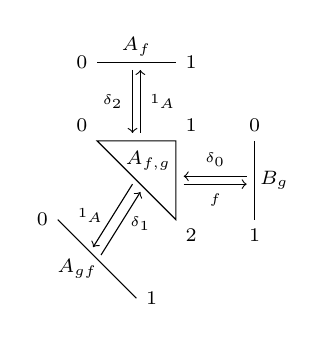
\begin{tikzpicture}
\path (0,0) node[above left,font=\scriptsize] (v00) {$0$};
\path (1,0) node[above right,font=\scriptsize] {$1$};
\path (1,-1) node[below right,font=\scriptsize] {$2$};
\draw[-] (0,0) -- (1,0) -- (1,-1) -- cycle;

\path (.65,-.250) node[font=\scriptsize] {$A_{f,g}$};

\path (0-.5,-1) node[left,font=\scriptsize] {$0$};
\path (1-.5,-2) node[right,font=\scriptsize] {$1$};
\draw[-] (0-.5,-1)-- (1-.5,-2);

\path (0,1) node[left,font=\scriptsize] (v00) {$0$};
\path (1,1) node[right,font=\scriptsize] {$1$};
\draw[-] (0,1)-- (1,1);

\path (2,0) node[above,font=\scriptsize] {$0$};
\path (2,-1) node[below,font=\scriptsize] {$1$};
\draw[-] (2,0)-- (2,-1);
\path (2.25,-.50) node[font=\scriptsize] {$B_{g}$};
\path (.5,1.20) node[font=\scriptsize] {$A_{f}$};
\path (.25-.5,-1.620) node[font=\scriptsize] {$A_{gf}$};
\path[->,font=\tiny] (.55,.1) edge node[right]{$1_A$} (.55,.9);
\path[->,font=\tiny] (.45,.9) edge node[left]{$\delta_2$} (.45,.1);
\path[->] (1.9,-.45) edge node[above,font=\tiny]{$\delta_0$} (1.1,-.45);
\path[->] (1.1,-.55) edge node[below,font=\tiny]{$f$} (1.9,-.55);
\path[->,font=\tiny] (.55-.5,.1-1.55) edge node[right]{$\delta_1$} (.55,.9-1.55);
\path[->,font=\tiny] (.45,.9-1.45) edge node[left]{$1_A$} (.45-.5,.1-1.45);
\end{tikzpicture}
\end{center}
\end{shaded}
\subsection*{(Co)simplicial replacement and (co)limits}
\begin{itemise}
\setlength{\parindent}{.25in}
\item $\scrc$ is a reflective subcategory of $\scrd$ if there is an adjunction
$\xymatrix@R=.3cm@C=1.5cm{
R:\scrd  \ar@<.6ex>[r]&
\scrc:i  \ar@{^{(}->}@<.4ex>[l]
}$
where the right adjoint $i$ is a full inclusion. Then the counit $Ri\nt 1_\scrc$ is a natural isomorphism%footnote:
\footnote{By Yoneda: $(RiX,Y)=(iX,iY)=(X,Y)$.}.
\item Given a simplicial set $X:\Delta^{\op}\to\Set$, we can form $\textbf{el}X\downarrow\Delta$, a category fibered in sets, called the \textbf{category of simplices}. The objects are just $\coprod X_n$, and
\[\textup{objects}(\textbf{el}X)=\coprod X_n,\quad \textup{hom}_{\textbf{el}X}(\sigma\in X_n,\sigma'\in X_m)=\left\{\textup{$[n]\overset{f}{\to}[m]$ in $\Delta$ sending $\sigma\overset{f^*}{\mapsfrom}\sigma'$}\right\}.\]
$\textup{el}X$ is fibered in sets over $\Delta$, with the fiber over $[n]$ just being $X_n$.
\begin{itemize}\squishlist
\setlength{\parindent}{.25in}
\item When $X=N\scrd$ is the nerve of $\scrd$, there is a functor $S:(\textup{el}N\scrd)^{\op}\to\scrd$, given by taking a chain of morphisms to its first object.
\item In this case, precomposition $S^*:\scrm^\scrd\to \scrm^{(\textup{el}N\scrD)^{\op}}$ is fully faithful, with left adjoint $\Lan_S$. Thus $S^*$ is the inclusion of a reflective subcategory, and the counit $\Lan_SS^*F\to F$ is an isomorphism for any $F:\scrd\to\scrM$.
\end{itemize}
\item Given a left Kan extension as at left, we have an equation of colimits:%footnote:
\footnote{By Yoneda: $C(\colim F,c)=C^A(F,\Delta c)=C^A(F,\Delta c\circ K)=C^B(\Lan_KF,\Delta c)=C(\colim \Lan_KF,c)$.}
\[\vcenter{\xymatrix{
A\ar[rd]_-{K}\ar[rr]^-{F}_-{}="arF"&%r1c1
&%r1c2
C\\%r1c3
&%r2c1
B\ar@{->}[ur]_{\Lan_KF}\ar@{=>}"arF";[]_-{\eta}&%r2c2
%r2c3
}}\qquad\implies\qquad  \colim_AF=\colim_D\Lan_KF\]
\end{itemise}
Suppose now that we have a functor $F:\scrd\to\scrm$. Then we have a diagram:
\[\xymatrix@!C{
&%r1c1
\Delta^{\op}
\ar[rd]^-{\Lan_\Sigma S^*F}
&%r1c2
\\%r1c4
(\textbf{el}N\scrd)^{\op}
\ar[ur]^-{\Sigma}
\ar[r]^-{S}
&%r2c1
\scrd
\ar[r]^-{F}
&%r2c2
\scrm%r2c4
}\]
And we find that
\[\colim_{\scrd}F=\colim_{\scrd}\Lan_S S^*F= \colim_{(\textbf{el}N\scrd)^{\op}}S^*F= \colim_{\Delta^{\op}}\Lan_\Sigma S^*F. \]
All that remains is to analyse the $\Lan_\Sigma S^*F$. We find that it is $B_\bullet (*,\scrd,F)$.
\end{5. The unreasonably effective (co)bar construction}
\begin{6. Homotopy limits and colimits, the theory}
\section*{Homotopy limits and colimits, the theory}
Suppose that $\scrm$ is a \textbf{simplicial model category}. We have an  endofunctor of the category of $\scrD$-shaped diagrams in $\scrM$:
\[\xymatrix@R=0mm{
\ar[r]^-{B(\scrD,\scrD,Q\DASH )}%Name of map
\scrM^\scrD&%Source
\scrM^\scrD\\%Target
F%x
\ar@{|->}[r]&
B(\scrD,\scrD,QF)%f(x)
%\ar@{}[ul];[l]|{\rotatebox{90}{\tiny$\in$}} \ar@{}[u];[]|{\rotatebox{90}{\tiny$\in$}} 
}\]
\begin{thm*}[6.1]
The pair 
\[B(\scrd,\scrd,Q\DASH ):\scrm^\scrd\to\scrm^d,\qquad B(\scrd,\scrd,Q\DASH )\nt Q\nt 1\]
is a left deformation for $\colim:\scrm^\scrd\to\scrm$, giving a left derived functor
\[\hocolim_\scrd:=\mathbb{L}\colim_\scrD \simeq B(*,\scrd,Q\DASH )\]
called the homotopy colimit.
\end{thm*}
\begin{itemise}
\setlength{\parindent}{.25in}
\item To obtain the expression $B(*,\scrd,Q\DASH )$, we note that
\[\colim_\scrd B(\scrd,\scrd,Q\DASH )=*\otimes _\scrd B(\scrd,\scrd,Q\DASH )=B(*\otimes _\scrd\scrd,\scrd,Q\DASH )=B(*,\scrd,Q\DASH ),\]
so it is enough to see that we indeed have a left deformation.
\item Using what we have, the proof is not too long.
\end{itemise}
\end{6. Homotopy limits and colimits, the theory}
\begin{7. Homotopy limits and colimits, the practice}
\section*{Homotopy limits and colimits, the practice}
\begin{itemise}
\setlength{\parindent}{.25in}
\item We \textbf{really} need a convenient category of spaces. We find one, and call it $\Top$.
\item Homotopy colimits are in general \textbf{not} colimits in the homotopy category. In fact, it is generally useless to think about diagrams in the homotopy category (and many of these don't even have colimits).
\item In $\Top$, we do not need the $Q$ in the above formula for homotopy colimits. \rednote{(Is this so for limits?)}
\item Formulas are given comparing pointed homotopy limits and colimits with unpointed ones.
\end{itemise}
\begin{thm*}[7.40]
There are natural isomorphisms
\[B(*,\scrd,F)\simeq N(\DASH /\scrd)\otimes_\scrd F\quad \textup{and}\quad C(*,\scrd,F)\simeq \left\{N(\scrd/\DASH),F\right\}^\scrd\]
\end{thm*}
\begin{proof}We'll be done if we know that $B(*,\scrd,\scrd)\cong N(-/\scrd)$, since then:
\[B(*,\scrd,F)\cong B(*,\scrd,\scrd\otimes _\scrD F)=B(*,\scrd,\scrd)\otimes _\scrD F=N(\DASH /\scrd)\otimes_\scrd F\]
Now \emph{the geometric realisation of a bisimplicial set} $X_{\bullet \bullet }$ is its diagonal. To see this, note that colimits in $\sSet$ are formed levelwise, so that the $n$-simplices of the realisation are:
\[|X_{\bullet \bullet }|_n=X_{\bullet n}\otimes _\Delta \Delta^\bullet _n=X_{\bullet n}\otimes _\Delta \Delta(n,\bullet )=X_{nn} \textup{\quad (by coYoneda).}\]
Now it happens that $B_\bullet (*,\scrd,\scrd(d,\DASH ))=N(d/\scrd)$. Viewing this as a bisimplicial set which is discrete in one variable, we have that its geometric realisation is the diagonal. This is just the simplicial set $N(d/\scrd)$, and this was a little tautological.
\end{proof}
\end{7. Homotopy limits and colimits, the practice}
\begin{8. Weighted limits and colimits}
\section*{Weighted limits and colimits}
\subsection*{Weighted limits in unenriched category theory}
\begin{itemise}
\setlength{\parindent}{.25in}
\item We can reformulate the concept of the limit/colimit of $F:\scrc\to\scrm$ as:
\[\scrm(m,\limit F)=\Set^\scrc(*,\scrm(m,F\DASH )),\ \qquad \,\scrm(\colim F,m)=\Set^\scrc(*,\scrm(F\DASH,m )).\]
A limit of $F$ \textbf{weighted} by $W:\scrC\to\Set$ is a representation
\[\scrm(m,\textstyle\limit^W\! F)=\Set^\scrc(W,\scrm(m,F\DASH )).\]
A colimit of $F$ \textbf{weighted} by $W:\scrC^{\op}\to\Set$ is a representation
\[\scrm(\textstyle\colim^W\! F,m)=\Set^{\scrc^{\op}}(W,\scrm(F\DASH,m )).\]
\item When enough limits exist, we calculate:
\begin{alignat*}{2}
\Set^\scrc(W,\scrm(m,F\DASH )) 
&\cong
\int_{c\in\scrc}\Set(Wc,\scrm(m,Fc))%
\\
&\cong
\int_{c\in\scrc}\scrm(m,Fc^{Wc})%
&\qquad&\text{($\scrm$ cotensored over $\Set$)}\\
\scrm(m,\textstyle\limit^W\! F)
&\cong
\scrm\left(m,\int_{c\in\scrc}Fc^{Wc}\right)%
&\qquad&\text{(representables preserve limits)}\\
% Left hand side
\textstyle\limit^W\! F
% Relation
&\cong
% Right hand side
\int_{c\in\scrc}Fc^{Wc}%
% Comment
&\qquad&\text{(Yoneda)}
\end{alignat*}
\begin{itemize}\squishlist
\setlength{\parindent}{.25in}
\item By Yoneda, $Fc=\limit^{\scrc(c,\DASH )}F$.
\item When $\scrm$ is complete, given 
\smash{$\vcenter{\xymatrix@R=3mm@C=1.5cm@!0{
&%r1c1
\scrm\\%r1c2
\scrc
\ar[ur]^-{F}
\ar[dr]_-{K}
&%r2c1
\\%r2c2
&%r3c1
\scrd%r3c2
}}$} there is a pointwise Kan extension:
\[\Ran_KF(d)=\int_{c\in\scrc} Fc^{\scrd(d,Kc)}= \textstyle\limit^{\scrd(d,K\DASH )}F.\]
\end{itemize}
\item We have a diagram 
${\xymatrix@1{
\textbf{el}W
\ar[r]^-{\Sigma}
&%r1c1
\scrc
\ar[r]^-{W}
&%r1c2
\Set%r1c3
}}$, and calculate:
\begin{alignat*}{2}
\textstyle\limit^W\!F
&=
\int_{c\in\scrc}Fc^{Wc}%
&\qquad&\text{(above)}\\
&=
\textup{eq} \left(\prod_{c}\prod_{Wc}Fc \rightrightarrows \prod_{c\to c'}\prod_{Wc}Fc'\right)%
&\qquad&\text{(expanding)}\\
&=
\textup{eq} \left(\prod_{(c,x)\in\ob(\textbf{el}W)} F\Sigma(c,x) \rightrightarrows \prod_{{{c\rightarrow c'}\atop{x\shortmapsto x'}}\in \arr(\textbf{el}W)}F\Sigma(c',x') \right)%
&\qquad&\text{(inspection)}\\
% Left hand side
% Relation
&=
% Right hand side
\limit_{\textbf{el}W}F\Sigma% Comment
&\qquad&\text{(formula for limits)}
\end{alignat*}
Thus we can write an unenriched wieghted limit as a standard limit over the category of elements of the weight.%footnote:
\footnote{$\textbf{el}W$ has objects pairs $(c,x)$ with $x\in Wc$, and $\Mor((c,x),(c',x'))$ those arrows $c\rightarrow c'$ under which $x\shortmapsto x'$.} This can be used to (finally) justify the formula:
\[\Ran_KF(d)=\lim\left(d/K\overset{U}{\to}\scrC\overset{F}{\to}\scrE\right).\]
\end{itemise}
\subsection*{Weighted limits and colimits}
\begin{itemise}
\setlength{\parindent}{.25in}
\item The category $\scrv\mathsf{Cat}$ of $\scrv$-categories and $\scrv$-functors is \textbf{closed symmetric monoidal}.
\begin{itemize}\squishlist
\setlength{\parindent}{.25in}
\item The tensor product of $\scrv$-categories takes the cartesian product on objects, but tensor products on hom-objects. To get a $\scrv$-category structure we repeatedly use the symmetry isomorphism in $\scrv$.
\item Given a \textbf{small} $\scrv$-category $\underline{\scrd}$ and any $\scrv$-category $\underline{\scrm}$, we can define $\underline{\scrm}^{\underline{\scrd}}$ with:
\begin{itemize}\squishlist
\setlength{\parindent}{.25in}
\item objects the $\scrv$-functors $\underline{\scrd}\to\underline{\scrm}$;
\item hom-objects via an \textbf{enriched} functor cotensor product:
\[\underline{\scrm}^{\underline{\scrd}}(F,G)=\int_{d\in\underline{\scrd}} \underline{\scrM}(Fd,Gd):=\textup{eq}\left(
\prod_{d}\underline{\scrm}(Fd,Gd)\rightrightarrows \prod_{d,d'}\underline{\scrv} \left(\underline{\scrd}(d,d'),\underline{\scrm}(Fd,Gd')\right)
\right)\]
\end{itemize}
We can describe the underlying set of ${\underline{\scrm}^{\underline{\scrd}}(F,G)}$ as follows. To give a point of this set is to give a map from $*$ to this equaliser, which is to give maps $\eta_d:*\to\underline{\scrm}(Fd,Gd)$ such that the following square commutes:
\[\vcenter{\xymatrix@R=6mm@C=45mm@!0{
&%r1c1
\underline{\scrm}(Fd,Gd)\otimes \underline{\scrd}(d,d')\ar[dr]^-{\DASH \circ (F\DASH)}
&%r1c2
\\%r1c3
\underline{\scrd}(d,d')
\ar[ur]^-{\eta_d\otimes 1}
\ar[dr]_-{1\otimes \eta_{d'}}
&%r2c1
&%r2c2
\underline{\scrm}(Fd,Gd')\\%r2c3
&%r3c1
\underline{\scrd}(d,d')\otimes \underline{\scrm}(Fd',Gd') \ar[uudr]_-{(F\DASH) \circ \DASH }&%r3c2
%r3c3
}}\]
That is, an element of the underlying set consists of unenriched data, with an enriched compatibility. \rednote{This appears to say that the underlying set is just the set of $\scrv$-natural transformations.} [If $\underline{\scrd}$ is the free $\scrv$-category on an unenriched category, $\underline{\scrM}^{\underline{\scrd}}(F,G)$ reduces to the unenriched end.]

\end{itemize}
\item We obtain a $\scrv$-\textbf{Yoneda lemma}:
\begin{lem*}
Given a small $\scrv$-category 
$\underline{\scrd}$, $d\in\underline{\scrd}$, and $F:\underline{\scrD}\to\underline{\scrv}$, the natural map is a $\scrv$-natural isomorphism:
\[Fd\overset{\cong}{\to}\underline{\scrv}^{\underline{\scrd}}(\underline{\scrd}(d,\DASH ),F).\]
\end{lem*}
\item We can define \textbf{weighted limits and colimits} of a $\scrv$-functor $\underline{\scrd}\to\underline{\scrv}$.
\begin{itemize}\squishlist
\setlength{\parindent}{.25in}
\item A limit of $F$ \textbf{weighted} by $W:\scrC\to\Set$ is a $\scrv$-natural isomorphism:
\[\underline{\scrm}(m,\textstyle\limit^W\! F)=\underline{\scrv}^{\underline{\scrd}}(W,\underline{\scrm}(m,F\DASH ))\quad \textup{(which equals $\limit^W\!\underline{\scrm}(m,F\DASH )$)}\]
\item A colimit of $F$ \textbf{weighted} by $W:\scrC^{\op}\to\Set$ is a representation
\[\underline{\scrm}(m,\textstyle\colim^W\! F)= \underline{\scrv}^{ \underline{\scrd}^{\op}}(W,\underline{\scrm}(F\DASH,m ))\quad \textup{(which equals $\limit^W\!\underline{\scrm}(F\DASH ,m)$)}\]
\end{itemize}
By these parenthesised comments, we see that enriched representable functors preserve limits and colimits appropriately.
\end{itemise}
\subsection*{Conical limits and colimits}
\begin{itemise}
\setlength{\parindent}{.25in}
\item Recall that when $\scrv$ is cocomplete and closed, there is an adjunction: 
\[\scrv[\DASH ]:\Cat\rightleftarrows\mathsf{\mathscr{V}Cat}:(\DASH )_0.\]
The objects of $\scrv[\scrc]$ are the those of $\scrc$, but $\scrv[\scrc](x,y):=\coprod_{\scrc(x,y)}*$.
\item An unenriched functor $\scrd\to\underline{\scrm}$ corresponds to an enriched functor $\scrv[\scrd]\to \scrm$. We may take the limit weighted by $*:\scrd\to\scrv$. A limit $\limit^*\!F$ of this form is a \textbf{conical limit}:
\[\underline{\scrm}(m,\textstyle\limit^*\!F)=
\underline{\scrv}^{\scrd}(*,\underline{\scrm}(m,F\DASH ))=
\textstyle\limit^*\underline{\scrm}(m,F\DASH )\]
\begin{itemize}\squishlist
\setlength{\parindent}{.25in}
\item Taking underlying sets, we see that $\limit^*\!F$ is in fact the ordinary limit of $F$ in $\scrm$.
\item The converse holds when $\underline{\scrm}$ is tensored over $\scrv$.
\end{itemize}
\end{itemise}
\subsection*{$\scrv$-completeness and $\scrv$-cocompleteness}
\rednote{I haven't really read this part.}
\subsection*{Homotopy (co)limits as weighted (co)limits}
\begin{itemise}
\setlength{\parindent}{.25in}
\item Suppose for simplicity that $\scrm$ is a simplicial model category will all objects cofibrant. Then
\[\hocolim_\scrd F=N(\DASH /\scrd)\otimes _\scrd F=\textstyle\colim^{N(\DASH /\scrd)}F.\]
That is, we have the defining universal property:
\[\underline{\scrm}(\hocolim_\scrd F,m)\cong\underline{\sSet}^{\scrd}(N(\DASH /\scrd),\underline{\scrm}(F\DASH ,m))\qquad 
\vcenter{\xymatrix@R=4mm@C=1.8cm@!0{
\hocolim F\ar[dd]
&%r1c3
\\%r1c3
&%r2c1
\makebox[0cm][r]{$\leftrightarrow$\quad }\scrd
\ar@/^1em/[r]^-{N(\DASH/\scrd)}_{}="1"
\ar@/_1em/[r]^{}="2"_-{\underline{\scrm}(F\DASH ,m)}&\underline{\sSet}%r2c2
\\%r2c3
m
\ar@{=>}"1";"2"
}}\]
That is, there is a universal simplicial natural transformation $N(\DASH /\scrd)\nt\underline{\scrm}(F\DASH ,\hocolim F)$. 
\begin{shaded}
I suppose that the idea is this. Suppose that one has chosen $d\in\scrd$ such that the objects with a map from $d$ look as simple as
\[\vcenter{\xymatrix@R=3mm@C=5mm{
&%r1c1
d\ar[ld]
\ar[rd]
&%r1c2
\\%r1c3
d'\ar[rr]
&%r2c1
&%r2c2
d''%r2c3
}}\textup{\quad so that\quad }d/\scrd\cong\Delta^2.\]
We may draw the simplices as:
\[0:\vcenter
{\def\objectstyle{\scriptstyle}
\xymatrix@R=8mm@C=8mm@!0{
d\ar@{=}[d]
&%r1c1
d\ar[d]
&%r1c2
d\ar[d]
\\%r1c3
d&%r2c1
d'&%r2c2
d''%r2c3
}}
\qquad 
1:
\vcenter{
\def\objectstyle{\scriptstyle}
\xymatrix@C=4mm@R=8mm@!0{
&%r1c1
d\ar[dr]
\ar@{=}[dl]
&%r1c2
&%r1c3
&%r1c4
d\ar[dr]
\ar[dl]
&%r1c5
&%r1c6
&%r1c7
d\ar[dr]
\ar@{=}[dl]
&%r1c8
\\%r1c9
d\ar[rr]
&%r2c1
&%r2c2
d'&%r2c3
d'\ar[rr]
&%r2c4
&%r2c5
d''&%r2c6
d\ar[rr]
&%r2c7
&%r2c8
d''%r2c9
}}\qquad 
2:
\vcenter{
\def\objectstyle{\scriptstyle}
\xymatrix@C=4mm@R=8mm@!0{
&&%r1c1
d\ar[drr]\ar[d]
\ar@{=}[dll]
\\%r1c9
d\ar[rr]
&%r2c1
&%r2c2
d'\ar[rr]
&%r2c4
&%r2c5
d''
}}\]
Now we obtain, from the universal natural transformation, a 2-simplex in the mapping simplicial set $\underline{\scrm}(Fd,H)$, where we write $H$ for $\hocolim F$.
\begin{itemize}\squishlist
\setlength{\parindent}{.25in}
\item The 0-simplices are genuine maps $Fd\to H$:
\begin{itemize}\squishlist
\setlength{\parindent}{.25in}
\item The first is supposed to be the inclusion of $Fd$ in $H$;
\item the second is that obtained by first mapping $Fd\to Fd'$ and then including $Fd'$ in $H$;
\item the second is that obtained by first mapping $Fd\to Fd''$ and then including $Fd''$ in $H$.
\end{itemize}
\item The 1-simplices are homotopies of maps $Fd\to H$, or maps $|\Delta^1|\times Fd\to H$. These are obtained by sliding along the homotopy used to identify $Fd$ with $Fd'$, $Fd'$ with $Fd''$ and $Fd$ with $Fd''$ respectively.
\item The 2-simplex is a homotopy between the composite of the first two 1-simplices and the third 1-simplex.
\end{itemize}
Any object $H'$ equipped with such maps, i.e.\ a natural transformation $N(\DASH /\scrd)\nt\underline{\scrm}(F\DASH ,H')$ admits a corresponding simplicial map from $\hocolim F$.
\end{shaded}
\item The \textbf{fat geometric realisation}: suppose that $\underline{\scrm}$ is a tensored and cotensored simplicial category. Then we can take the fat geometric realisation by taking tensor products with the cosimplicial simplicial set $N(\Delta/\DASH ):\Delta\to\sSet$. This maps to the Yoneda embedding, so that there is a natural map from the fat geometric realisation to the geometric realisation, called the \textbf{Bousfield Kan map}. If $X$ is Reedy cofibrant, this is a weak equivalence.

To describe the map to the Yoneda embedding, one takes an $m$-simplex $[n_0]\to[n_1]\to\cdots \to[n_m]\to[n]$, and looks at the images in $[n]$ of the last vertices in each of $[n_0]$, $[n_1]$, etc. This gives a map $[m]\to[n]$, i.e.\ an $m$-simplex of $\Delta^n$.
\end{itemise}
\subsection*{Balancing bar and cobar constructions}
It is calculated, that when $\scrm$ is a simplicial model category, that for a diagram $F:\scrd\to\scrm$:
\[\underline{\scrm}(B(*,\scrd,F),m)\cong \int_{n\in\Delta}\prod_{\vec d\in (N\scrd)_n}\underline{\scrm}(Fd_0,m)^{\Delta^n}.\]
\begin{shaded}
That is like saying: to map $\phi$ out of the bar construction, one needs to give, for each $\vec d\in (N\scrd)_n$, a map $\Delta^n\times Fd_0\to m$. This map is of course supposed to be the restriction of $\phi$ to the span inside the bar construction starting with $d_0$ corresponding to $\vec d$. 
\end{shaded}
\noindent The point is that the right hand expression looks quite a lot like $C(*,\scrd^{\op},\underline{\scrm}(F\DASH ,m))$, but the two are not the same. A point in this cobar construction is (by example 8.49), a homotopy coherent choice of maps $Fd\to m$.
\rednote{There's some foreshadowing going on here, but I'm not really getting the point.}
\end{8. Weighted limits and colimits}
\end{document}
















